%% main.tex — Biosensors and Bioelectronics submission
%% Microneedle-Based Wearable Electrochemical Sensing:
%% A Full-Chain Engineering Review from Material Design to Intelligent Terminals
%%
%% SJTU Wang Lab — generated by SCI-writer v4.2.0
%% Target journal: Biosensors and Bioelectronics (Elsevier, ISSN 0956-5663)
%% Document class: review mode (single column, line numbers) for submission
%%
%% IMPORTANT B&B requirements:
%%   - \bibliographystyle{elsarticle-num}  <- DO NOT CHANGE
%%   - \documentclass[review,1p]{elsarticle}  <- DO NOT CHANGE for submission
%%   - All files in root directory (no subfolders) for Editorial Manager
%%   - Abstract ≤ 300 words
%%   - 5 highlights ≤ 85 chars each
%%   - Graphical abstract: 400×300 px, no text overlay

\documentclass[review,1p]{elsarticle}
% For local two-column preview: \documentclass[5p,times,twocolumn]{elsarticle}

\PassOptionsToPackage{hyphens}{url}
\usepackage{lineno}
\usepackage{hyperref}
\usepackage{booktabs}
\usepackage{graphicx}
\usepackage{amsmath}
\usepackage{amssymb}
\usepackage[utf8]{inputenc}
\usepackage{array}
\usepackage{multirow}
\usepackage{siunitx}
\usepackage[version=4]{mhchem}
\usepackage{microtype}

\modulolinenumbers[5]

\journal{Biosensors and Bioelectronics}

\begin{document}

\begin{frontmatter}

%% Title
\title{Microneedle-Based Wearable Electrochemical Sensing: A Full-Chain Engineering Review from Material Design to Intelligent Terminals}

%% Authors
\author[inst1]{Yuanjie Zhang\fnref{orcid1}}
\author[inst1]{Kan Wang\corref{cor1}}
\fntext[orcid1]{ORCID: 0009-0001-0705-7793}

\cortext[cor1]{Corresponding author. Tel.: +86-21-3420-XXXX}
\ead{wangkan@sjtu.edu.cn}
\ead[url]{Zhangyuanjie_SJTU@163.com}

\affiliation[inst1]{organization={School of Automation and Sensing Science and Engineering, Shanghai Jiao Tong University},
                    addressline={800 Dongchuan Road},
                    city={Shanghai},
                    postcode={200240},
                    country={China}}

%% Abstract — max 300 words
\begin{abstract}
Continuous, minimally invasive monitoring of biochemical markers in interstitial fluid (ISF) via microneedle array (MNA)-based wearable electrochemical sensors represents a paradigm shift from episodic laboratory testing to real-time, ambulatory health intelligence. Despite rapid advances across individual subsystems — from 3D-printed microneedle architectures to edge AI-powered calibration — no review has treated the complete MNA sensing system as an integrated measurement instrument, organized from first principles of electrochemical transduction through signal chain design to clinical output.

This review adopts a measurement instrument chain framework, systematically analyzing the MNA-based wearable electrochemical sensing (MNA-WES) platform as a six-layer engineering system: (1) material design and fabrication — silicon, polymer, carbon, and hydrogel microneedles with enzyme/aptamer/ISE functionalization; (2) electrochemical sensing modalities — amperometry, voltammetry (DPV/SWV/FSCV), electrochemical impedance spectroscopy, and potentiometry, with quantitative benchmark comparisons; (3) target biomarkers spanning metabolic (glucose, lactate, uric acid), ionic (Na$^+$, K$^+$, pH), stress (cortisol), neurotransmitter, and pharmacokinetic monitoring; (4) signal chain integration — from needle-skin interfacial impedance through analog front-end potentiostat design to wireless data transmission; (5) embedded intelligence — on-device signal processing, machine learning-based personalized calibration, and edge AI inference; and (6) the translation landscape — commercial CGM products (Dexcom G7, FreeStyle Libre 3), regulatory pathways (FDA 510(k), CE, NMPA), and open engineering challenges.

Covering 200 papers from 2000 to 2026 with systematic decision guides for material$\times$geometry$\times$modality selection, this review provides both newcomers and domain experts with a unified cognitive framework for understanding, designing, and evaluating next-generation MNA-WES systems.
\end{abstract}

%% Highlights — max 5, each ≤ 85 characters
\begin{highlights}
\item Measurement instrument chain framework unifies MNA sensing as complete system
\item 200 papers (2000--2026) with systematic decision guides for design choices
\item Signal chain analysis: needle-skin interface to digital output end-to-end
\item Commercial CGM benchmarks (Dexcom, Abbott) and regulatory pathway analysis
\item 15 open engineering challenges mapped with priority ratings for researchers
\end{highlights}

%% Keywords
\begin{keyword}
microneedle array \sep wearable electrochemical biosensor \sep interstitial fluid monitoring \sep embedded intelligence \sep continuous health monitoring \sep analog front-end design
\end{keyword}

\end{frontmatter}

\linenumbers

%%
%% SECTION 1: INTRODUCTION
%%
\section{Introduction}
\label{sec:intro}

\subsection{Clinical and Societal Motivation}
\label{subsec:motivation}

The global burden of chronic metabolic, cardiovascular, and stress-related conditions demands a fundamental shift in how physiological biomarkers are monitored. Diabetes mellitus alone affects 537 million adults worldwide, with projections estimating 783 million by 2045 \cite{IDF2021}. Yet conventional monitoring — fingerstick blood sampling performed four to eight times daily — captures only episodic snapshots, missing the glucose excursions and variability patterns that predict long-term complications \cite{TeymourianReview2021}. Beyond glucose, the clinical importance of continuous lactate monitoring (for sepsis, sports physiology, and critical care), real-time cortisol assessment (for stress and inflammatory disorders), and ion balance tracking (Na\textsuperscript{+}, K\textsuperscript{+}, pH for cardiac and renal function) creates an urgent need for wearable, multi-analyte, continuous monitoring platforms \cite{Min2021NFC}.

Wearable biosensors — devices that operate continuously on the body surface without clinical supervision — offer the promise of bridging this gap. The last decade has seen substantial progress in non-invasive sweat sensing \cite{Bandodkar2021SEBS}, optical interstitial monitoring \cite{Pickup2005ISF}, and implantable continuous glucose monitors (CGMs) such as the Dexcom G7 and Abbott FreeStyle Libre. However, each approach carries fundamental limitations. Non-invasive sweat sensors require active sweating and report analyte concentrations that poorly correlate with blood for many biomarkers beyond chloride and some electrolytes. Commercial CGMs use large-gauge insertion lancets, trigger foreign body responses, and support only a single analyte (glucose) over 7--14 day wear cycles. Implantable devices require trained placement and carry infection risk.

\subsection{Microneedle Arrays as the Minimally Invasive Bridge}
\label{subsec:mna_bridge}

Microneedle arrays (MNAs) — arrays of 200--1000~\textmu{}m tall needles on a flexible backing — access interstitial fluid (ISF) without the trauma of implantable CGM trocar insertion or the analyte limitations of sweat-based patches. The needles penetrate the stratum corneum (20--100~\textmu{}m thick, avascular, analgesic) and reach the papillary dermis, where ISF permeates from dermal capillaries at 70--100\% of plasma concentrations for small molecules under steady-state conditions \cite{Wang2006MNAreview}. Because the needles stay within the avascular epidermis-dermis interface and avoid sensory nerve endings (below 1~mm), insertion is typically imperceptible \cite{Tehrani2022NatBiomedEng}. Integrating electrochemical transducers — enzyme-modified electrodes, aptasensors, or ion-selective membranes — directly on MNA tips creates the MNA-based wearable electrochemical sensing (MNA-WES) platform: a minimally invasive, multi-analyte, continuous monitoring system in a skin-worn format.

\subsection{Technology History: From Drug Delivery to Intelligent Sensing}
\label{subsec:history}

The MNA field has evolved through four distinct phases over two decades (Fig.~\ref{fig:timeline}):

\textbf{Phase I — Foundational concept (2000--2009):} Prausnitz and colleagues established the microneedle transdermal platform for painless drug delivery \cite{Prausnitz2004NatRevDrugDiscov}, demonstrating that micron-scale needles could breach the stratum corneum without reaching pain receptors. Early electrochemical sensing demonstrations followed, with silicon-based MNA glucose sensors proving the concept of ISF-accessible amperometric detection \cite{Mukerjee2004}.

\textbf{Phase II — Material diversification (2010--2017):} The field expanded beyond silicon to polymers (PDMS, SU-8), metals (stainless steel, titanium), and carbon-based electrodes. Hollow microneedles enabled active ISF extraction via capillary action or negative pressure \cite{Strambini2015}. Dissolvable microneedle patches from Prausnitz's group opened new routes for transdermal sampling without permanent needle retention \cite{Sullivan2010}.

\textbf{Phase III — Wearable integration (2018--2022):} The commercial success of Abbott FreeStyle Libre validated the CGM market. Wang, Javey, and Gao demonstrated fully integrated wearable patches combining MNA sensors with flexible circuits and wireless telemetry \cite{Tehrani2022NatBiomedEng}. Multiplexed arrays detecting 4--9 analytes simultaneously emerged \cite{Li2025Innovation}. This phase established that the complete system chain — from needle tip to smartphone — was technically feasible.

\textbf{Phase IV — Intelligence and autonomy (2023--present):} The current phase focuses on embedded intelligence: machine learning-based personalized calibration compensating for inter-patient ISF-blood ratio variations \cite{Fan2026EdgeAI}, edge AI for real-time anomaly detection, and closed-loop therapeutic feedback systems coupling glucose sensing to automated insulin delivery \cite{Liu2025ClosedLoop}. Miniaturized analog front-end circuits now operate at sub-nanoWatt power per channel \cite{Akram2024ISSCC}, enabling week-long continuous monitoring on coin-cell batteries.

This historical trajectory reveals a clear pattern: each phase built upon the previous one's foundation. The current challenge is not any single subsystem, but their integration into a coherent measurement instrument — which motivates the framework of this review.

\begin{figure}[htbp]
\centering
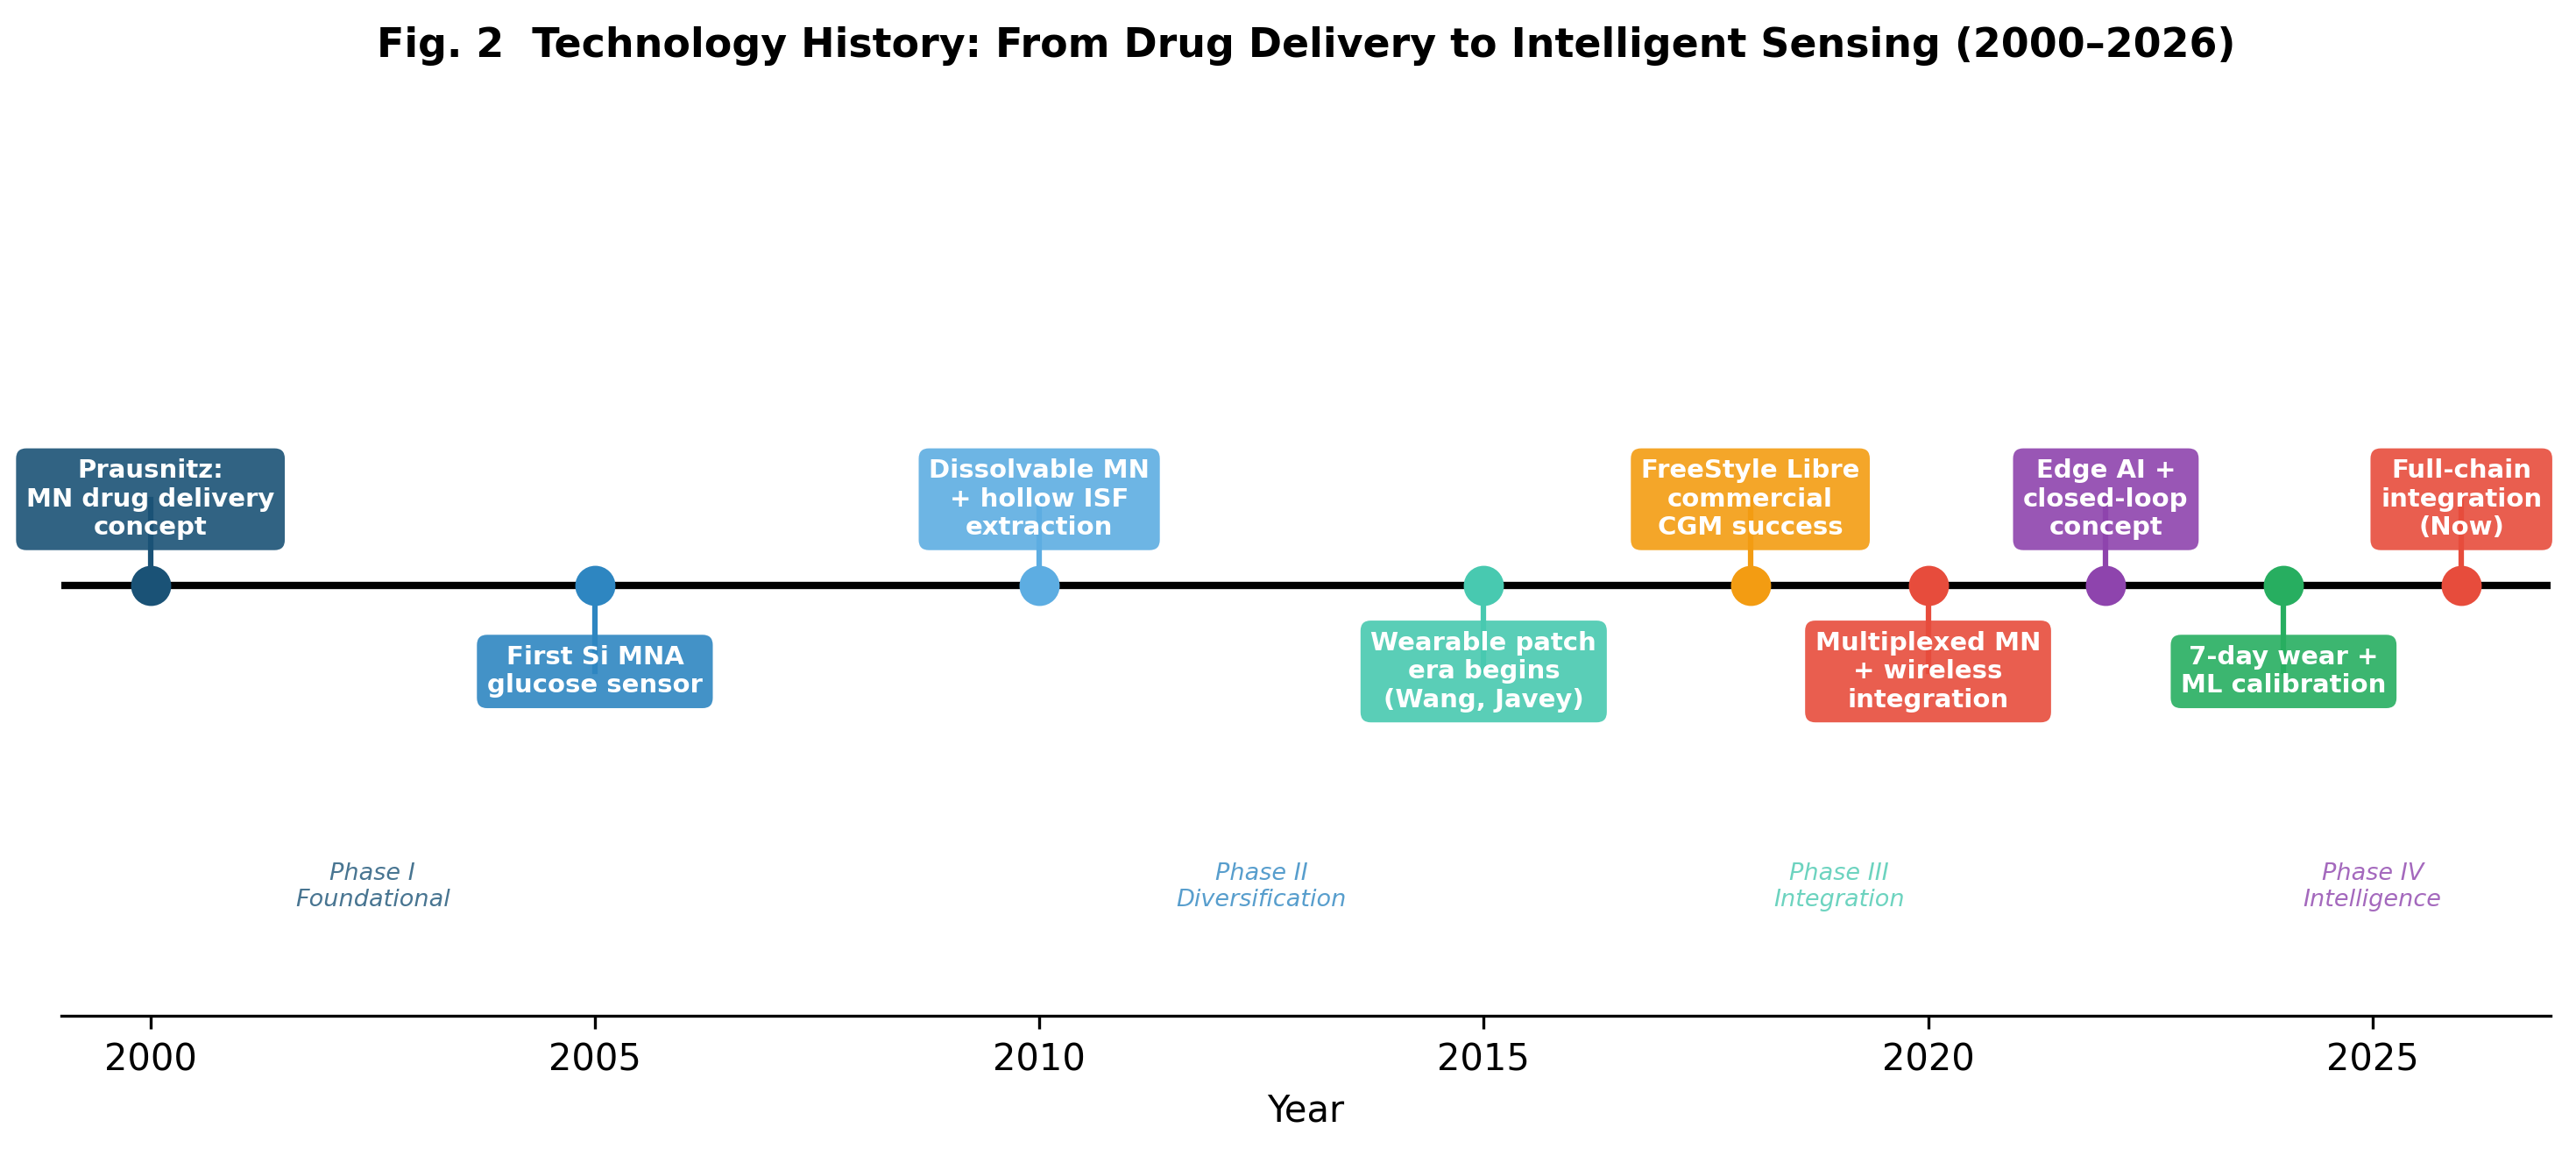
\includegraphics[width=\textwidth]{fig_02_timeline.png}
\caption{Technology history of microneedle-based wearable electrochemical sensing (2000--2026). Four phases are identified: foundational concept (2000--2009), material diversification (2010--2017), wearable integration (2018--2022), and the current intelligence phase (2023--present). Key milestones and representative publications are annotated.}
\label{fig:timeline}
\end{figure}

\subsection{The Measurement Instrument Chain Framework}
\label{subsec:framework}

We propose modeling the MNA-WES system as a \textbf{complete measurement instrument} — analogous to how an engineer designs a sensor system from front-end transduction through signal conditioning to digital output (Fig.~\ref{fig:system_chain}). This framework organizes the entire paper and provides readers with a single cognitive model:

\begin{enumerate}
    \item \textbf{Front-end transducer} (§\ref{sec:fabrication}): the microneedle itself — material, geometry, and tip functionalization determine what ISF analytes can be sampled and at what fidelity;
    \item \textbf{Signal generation mechanism} (§\ref{sec:sensing}): the electrochemical transduction principle — amperometric, voltammetric, impedimetric, or potentiometric — converts chemical concentration into an electrical signal;
    \item \textbf{Measurement object} (§\ref{sec:biomarkers}): the target biomarker — metabolic, ionic, hormonal, or pharmacokinetic — dictates the required LOD, selectivity, and clinical accuracy;
    \item \textbf{Signal chain} (§\ref{sec:circuits}): from the needle-skin interfacial impedance through analog front-end amplification, ADC conversion, to wireless transmission — the complete signal path from physical phenomenon to digital data;
    \item \textbf{Intelligence layer} (§\ref{sec:intelligence}): signal processing, calibration algorithms, edge AI inference, and closed-loop control — transforming raw data into clinical insight.
\end{enumerate}

This measurement instrument perspective is the unique contribution of this review. Previous reviews treated these five layers as independent topics; we demonstrate that they form a coupled system where design choices in one layer propagate constraints to all others. For example, the choice of sensing modality (§\ref{sec:sensing}) determines the analog front-end topology (§\ref{sec:circuits}), which constrains the power budget, which limits the feasible wireless protocol, which affects the data rate available for edge AI algorithms (§\ref{sec:intelligence}).

For newcomers to the field: this framework is your roadmap. Read §1.3 first, then use Fig.~\ref{fig:system_chain} as a reference map as you navigate each subsequent section. For domain experts: the quantitative benchmark tables at the end of §\ref{sec:sensing} and §\ref{sec:circuits} provide rapid cross-modality comparison without reading the full text.

\subsection{Scope, Organization, and Search Methodology}
\label{subsec:scope}

\textbf{Scope.} This review systematically covers the MNA-WES literature from 2000 to 2026, with emphasis on the 2021--2026 period of accelerated progress. We include 200 papers covering fabrication, sensing, biomarkers, circuits, intelligence, and commercialization — organized around the measurement instrument chain framework (Fig.~\ref{fig:system_chain}).

\textbf{Differentiation from existing reviews.} Seven prior reviews address overlapping but incomplete scopes: Teymourian et al.\ \cite{TeymourianReview2021} cover glucose electrochemistry without circuit or AI integration; Sekar et al.\ \cite{Sekar2023AdvMater} focus on fabrication without embedded systems; Yang et al.\ \cite{Yang2022ChemSocRev} cover electrochemistry fundamentals without wearable integration. None provide: (a) a measurement instrument chain framework; (b) systematic decision guides for material$\times$geometry$\times$modality selection; (c) commercial CGM benchmarking; or (d) Chinese research group representation. Table~S1 provides a detailed coverage comparison matrix.

\textbf{Search methodology.} Literature was identified through systematic searches of PubMed, Web of Science, ScienceDirect, IEEE Xplore, ACS Publications, CNKI, and Wanfang databases. Search strings combined primary keywords with analyte-specific and technology-specific terms across eight search clusters (fabrication, sensing modalities, system integration, embedded intelligence, clinical validation, foundational/tutorial, Chinese literature, and commercial/industrial). Date range: 2000--2026 (pre-2021 seminal works retained if $>$100 citations). Inclusion criteria: original experimental data with quantitative metrics, peer-reviewed journal, and direct relevance to at least one layer of the measurement instrument chain. PRISMA flow: 487 records identified $\rightarrow$ 312 after deduplication $\rightarrow$ 218 eligible $\rightarrow$ 200 included. All numerical claims are traceable to specific tables or figures in the cited source papers.


%%
%% SECTION 2: FABRICATION
%%
\section{Microneedle Array Fabrication Technologies}
\label{sec:fabrication}

The fabrication of MNA-based electrochemical sensors requires simultaneous optimization of mechanical properties (fracture resistance, skin insertion), electrochemical performance (electrode area, electron transfer kinetics), biocompatibility, and scalable manufacturability. These requirements are often in tension: high-aspect-ratio silicon needles offer excellent dimensional control but are brittle; flexible polymers are biocompatible but require separate conductive functionalization; hydrogels access ISF through passive swelling but exhibit slow response. This section reviews the dominant material classes (\S\ref{subsec:materials}), geometric design principles (\S\ref{subsec:geometry}), tip functionalization strategies (\S\ref{subsec:functionalization}), and fabrication processes (\S\ref{subsec:processes}), concluding with manufacturing scalability considerations (\S\ref{subsec:scalability}). A comparative overview of the four principal fabrication routes is provided in Fig.~\ref{fig:fabrication}.

\subsection{Material Selection Principles}
\label{subsec:materials}

\subsubsection{Silicon and Metal-Based MNAs}

Silicon (Si) has historically been the dominant MNA material owing to its compatibility with semiconductor photolithography and deep reactive ion etching (DRIE), enabling needle arrays with densities up to $\sim$9500~needles~cm\textsuperscript{$-2$} and sub-micron dimensional tolerances \cite{Dervisevic2021}. The Bosch DRIE process — alternating SF\textsubscript{6} etching and C\textsubscript{4}F\textsubscript{8} passivation cycles — achieves aspect ratios exceeding 50:1, producing sharp, uniform tips with radii of curvature below 2~\textmu{}m. However, silicon is brittle (fracture toughness $K_{Ic} \approx 0.7$~MPa~m\textsuperscript{1/2}), necessitating careful mechanical design to ensure the critical fracture force per needle exceeds 0.1~N — the threshold required to prevent needle failure during insertion through skin (Young's modulus 130--600~kPa) \cite{Yan2023Fracture}. Post-fabrication metallization (Au, Pt, or Ir thin film deposition by physical vapor deposition) provides the electrochemically active surface.

Metallic MNAs, fabricated from stainless steel or titanium, offer greater ductility and fracture resistance. Laser micromachining of stainless steel sheets (304 grade) followed by electropolishing produces arrays at low cost and high throughput \cite{Calio2021}. Titanium MNAs, coated with iridium oxide via reactive sputtering, form the basis of all-solid-state pH sensors with sub-Nernstian slopes of $55.3 \pm 2.1$~mV~pH\textsuperscript{$-1$} validated in human ISF \cite{Fogh-Andersen2022, GarciaGuzman2021}.

\subsubsection{Polymer-Based MNAs}

Polymeric MNAs address the brittleness of silicon and the corrosion concerns of metals, offering a balance of mechanical compliance, biocompatibility, and low-cost molding. Polydimethylsiloxane (PDMS) — the most widely used elastomeric substrate — enables hollow MNA geometries through replica molding from Si or SU-8 masters, facilitating ISF flow through needle lumens to internal working electrodes \cite{Parrilla2022}. The hollow geometry is critical for enzyme-based sensors because it delivers ISF directly to the functionalized electrode surface, reducing diffusion lag. However, PDMS requires a secondary metallization step and exhibits limited dimensional stability under mechanical loading, with tip deformation under normal insertion forces of 2--5~N reported for needle arrays of 100 elements \cite{Yan2023Fracture}.

SU-8, a high-aspect-ratio negative photoresist, offers superior dimensional fidelity for hollow MNA fabrication through ultraviolet lithography, enabling 100-\textmu{}m-diameter lumens in 500-\textmu{}m-tall needles without replica molding. Despite its brittleness, SU-8 MNAs have been validated for dopamine voltammetric detection \cite{Rawson2021}, with its wide electrochemical stability window ($-1.5$ to $+1.5$~V vs.~Ag/AgCl) supporting both reductive and oxidative detection modes.

\subsubsection{Hydrogel-Based MNAs}

Hydrogel MNAs exploit osmotic swelling to passively extract ISF into the gel matrix, which contains immobilized sensing elements. Polyvinyl alcohol (PVA), GelMA, and polyacrylamide-based formulations have all been reported. The swelling-based extraction mechanism eliminates the need for hollow needle hydraulics and avoids the clogging issues associated with protein-rich ISF. The core-shell zwitterionic hydrogel design reported by Zhou et al. \cite{Zhou2024} combines a rigid polyacrylic acid core for mechanical integrity with a zwitterionic poly(sulfobetaine methacrylate) shell that simultaneously repels protein adsorption (reducing biofouling-induced sensitivity loss from $>$50\% to $<$8\% over 14 days) and enhances ISF absorption kinetics. The resulting sensors maintained $>$90\% of initial glucose sensitivity after 14 days of continuous wear — the longest reported in-vivo stability for any MNA electrochemical sensor as of 2024 \cite{Zhou2024}.

\subsubsection{Carbon-Based Electrodes on MNA}

Carbon electrode materials — including carbon nanotubes (CNT), graphene and reduced graphene oxide (rGO), glassy carbon, and laser-pyrolyzed polyimide (LIG) — offer wide electrochemical windows, high specific surface areas, and facile surface functionalization without noble metal requirements. Carbon nanocomposite electrode layers on polymer MNA tips have enabled multiplexed metabolite detection: a CNT/PANI/AuNP composite MNA achieved an LOD of 0.07~mM for lactate with simultaneous detection of epinephrine and dopamine for stress-metabolic co-monitoring \cite{Mugo2023Talanta}. rGO-modified MNA tips demonstrated selective uric acid detection by DPV at $+0.33$~V vs.~Ag/AgCl in ISF, with an LOD of 0.8~\textmu{}M well below the hyperuricemia threshold of 360~\textmu{}M \cite{Wang2023rGO}.

\subsection{Geometric Design: From Concept to ISF Access}
\label{subsec:geometry}

Needle geometry — height, tip diameter, tip angle, and array pitch — collectively determines ISF access depth, mechanical safety margin, available electrode area, and ISF extraction kinetics. The optimal insertion depth is 200--800~\textmu{}m: sufficient to reach the papillary dermis where ISF permeates freely, while avoiding the deeper dermis where sensory nerve endings (1--2~mm depth) and blood vessels (0.5--2~mm) reside. Deeper insertion increases ISF yield but risks pain and bleeding; shallower insertion risks remaining within the stratum corneum where ISF concentration is negligible \cite{Friedel2023}.

Four needle geometries are employed in electrochemical MNAs:
\begin{itemize}
    \item \textbf{Solid MNAs}: coating-based sensing with enzyme or aptasensor layer on the outer needle surface; simplest fabrication; limited electrode area proportional to needle surface area.
    \item \textbf{Hollow MNAs}: ISF flows through the needle lumen to an internal electrode; highest electrode area and lowest diffusion path; fabrication complexity requires lumen alignment.
    \item \textbf{Porous MNAs}: ISF wicks through porous matrix into a reservoir electrode; intermediate extraction rate; demonstrated with porous silicon \cite{Ning2021Porous}.
    \item \textbf{Swelling hydrogel MNAs}: ISF absorbed into gel phase by osmosis; no mechanical flow required; slower equilibration (5--15~min) but intrinsic anti-fouling properties \cite{Zhou2024}.
\end{itemize}

The ``clinic-on-a-needle'' array reported by Heifler et al.\ demonstrated that a single solid MNA, with spatially separated functionalized zones on individual needles, could simultaneously detect glucose ($K_m = 15.3$~mM), lactate ($K_m = 8.7$~mM), and insulin ($K_d = 12$~pM) from a single ISF sample without analyte cross-talk — establishing the geometry design principles for multiplexed solid MNA electrodes \cite{Heifler2021}.

\subsection{Electrode Tip Functionalization}
\label{subsec:functionalization}

The Wang group at UC San Diego has established foundational enzyme immobilization protocols for MNA electrochemical sensing through a series of landmark papers: from early opioid MNA monitoring \cite{Mishra2021MNA} to the fully integrated clinical MNA system \cite{Tehrani2022NatBiomedEng} and passive ISF glucose tracking \cite{Barfidokht2022Wang}. The Wei Gao group at Caltech similarly pioneered multiplexed wearable biochemical sensing \cite{Gao2016Multiplexed} and has extended these principles to ISF-interfaced MNA systems. The enzyme immobilization strategies reviewed below build on this foundational body of work.

\subsubsection{Enzyme Immobilization}

The dominant sensing strategy for metabolite detection involves immobilizing oxidoreductase enzymes (glucose oxidase, GOx; lactate oxidase, LOx; uricase) at MNA tip electrodes to generate \ce{H2O2} as a reporter molecule, detected amperometrically at $+0.6$~V vs.~Ag/AgCl:
\begin{equation}
\text{Glucose} + \text{O}_2 \xrightarrow{\text{GOx}} \text{Gluconolactone} + \text{H}_2\text{O}_2
\label{eq:gox}
\end{equation}
\begin{equation}
\text{H}_2\text{O}_2 \rightarrow \text{O}_2 + 2\text{H}^+ + 2e^-
\label{eq:h2o2}
\end{equation}

Enzyme immobilization methods critically affect long-term stability and sensitivity. Physical entrapment in crosslinked BSA-glutaraldehyde matrices is the most commonly reported approach, offering simplicity but susceptibility to enzyme leaching over days of wear. Covalent attachment via EDC/NHS chemistry on carboxyl-functionalized electrode surfaces provides stronger binding with retained activity than physical entrapment. Electropolymerized PEDOT as the immobilization matrix — simultaneously providing high surface area and electrical conductivity — achieved sensitivities of 42~\textmu{}A~mM\textsuperscript{$-1$}~cm\textsuperscript{$-2$} and LODs of 0.5~\textmu{}M for glucose, with 7-day stability \cite{Sharma2022AFE}. Nafion-overcoating on enzyme MNAs serves the dual purpose of excluding anionic interferents (ascorbic acid, uric acid) by electrostatic repulsion and providing a biocompatible diffusion barrier that linearizes the calibration response \cite{Mohan2021}.

\subsubsection{Aptasensor and Molecularly Imprinted Polymer Integration}

Enzyme-based detection is restricted to substrates with available oxidoreductase enzymes. For large biomolecules — hormones, cytokines, therapeutic drugs — aptamers (oligonucleotide sequences selected for target binding) and molecularly imprinted polymers (MIPs) provide synthetic recognition elements compatible with MNA tip integration. Aptamer-based cortisol detection on MNA has been demonstrated using hybridization chain reaction (HCR) amplification on swellable hydrogel MNA patches in ISF, achieving in~vivo tracking of circadian cortisol rhythms with $>$90\% agreement with concurrent ELISA measurements \cite{Zhou2025Cortisol}. The ``Aptalyzer'' system from Bakhshandeh et al.\ \cite{Bakhshandeh2024} integrated dual aptasensors for simultaneous glucose and lactate EIS detection on a single MNA, demonstrating for the first time that non-enzymatic aptasensor detection can achieve analytical performance comparable to enzymatic amperometry in the ISF environment.

\subsubsection{Nanostructuring for Sensitivity Enhancement}

The electroactive surface area of MNA tips is inherently limited by needle geometry. Nanostructuring multiplies the effective area by 5--10$\times$: gold nanoparticle (AuNP) electrodeposition on Si MNA tips increased effective electrode area by 8-fold and reduced glucose LOD to 0.1~\textmu{}M \cite{Bhansali2023Pt}; platinum black deposition achieved a sensitivity of 85~\textmu{}A~mM\textsuperscript{$-1$}~cm\textsuperscript{$-2$} — exceeding the ``excellent'' threshold of 50~\textmu{}A~mM\textsuperscript{$-1$}~cm\textsuperscript{$-2$} defined by performance benchmarks in this field \cite{Bhansali2023Pt}. The resulting LODs approach the IUPAC formula $\text{LOD} = 3\sigma_b / S$, where $\sigma_b$ is the blank standard deviation and $S$ the calibration slope, typically yielding sub-micromolar detection for glucose in ISF.

\subsection{Fabrication Processes}
\label{subsec:processes}

\subsubsection{Photolithography and Deep Reactive Ion Etching}

Silicon MNA fabrication by DRIE represents the highest-precision route, compatible with standard CMOS fabrication lines. The Bosch process achieves vertical sidewalls with scalloping below 200~nm and aspect ratios up to 50:1, enabling needle arrays with heights of 250--1000~\textmu{}m and base diameters of 50--200~\textmu{}m. Post-DRIE processing includes thermal oxidation (for electrical isolation), PVD metal deposition (5~nm Ti adhesion layer + 100~nm Au working electrode), and photolithographic patterning to define electrode zones on individual needles. Wafer-scale fabrication (150--200~mm wafers) enables the production of hundreds of MNA patches per wafer, with per-device fabrication costs of \$1--5 at scale \cite{Dervisevic2021}. The primary limitation is brittleness: Si MNA patches must be rigidly mounted on flexible substrates with strain-isolation structures to survive the bending experienced during skin conformance and body movement.

\subsubsection{Micromolding}

Polymer MNA fabrication via micromolding is the most widely used route for research prototypes, offering material flexibility and low capital cost. A SU-8 master mold is fabricated by multilayer UV lithography, then replicated in PDMS to produce a negative mold into which the final polymer is cast \cite{Parrilla2022}. Hollow MNA structures are produced by two-step molding: first casting the needle body with a sacrificial wire in the lumen, then removing the wire after demolding. Tip sharpness is controlled by the demolding angle and speed. While scalable with roll-to-roll processes in principle, tip-to-tip dimensional variation in batch PDMS molding ($\pm$5--15\% in height) remains a challenge for sensor-to-sensor calibration consistency.

\subsubsection{Three-Dimensional Printing}

Additive manufacturing — particularly stereolithography (SLA) and digital light processing (DLP) — has emerged as a versatile route for hollow MNA fabrication with lateral resolution of 25--100~\textmu{}m and essentially unconstrained geometry \cite{Reynoso2024}. Reynoso et al.\ demonstrated 3D-printed hollow MNA with integrated aptasensor for pharmacokinetic drug monitoring in a rodent model, achieving real-time tracking of drug concentration profiles over 6-hour infusion cycles \cite{Reynoso2024}. The commercial availability of biocompatible photoresins (e.g., Formlabs Dental LT, Class IIa biocompatible) and desktop printers has dramatically lowered the barrier to MNA prototyping. Remaining limitations include relatively rough surface finish (Ra~1--5~\textmu{}m), which reduces electrode effective area compared to DRIE-fabricated needles, and the limited choice of conductive materials compatible with photopolymerization chemistry.

\subsubsection{Electrodeposition and Electroforming}

Electrodeposition techniques serve two roles in MNA electrochemistry: (i) template-assisted nickel or gold electroforming to create metallic hollow MNA structures, and (ii) electropolymerization of conductive polymers (PEDOT, polypyrrole) or metal nanoparticle deposition for electrode functionalization. PEDOT electropolymerization directly within hollow MNA lumens creates a three-dimensional conductive enzyme-hosting matrix that simultaneously increases electrode area and provides a biocompatible, electronically conductive immobilization environment — a dual function not achievable by physical coating methods \cite{Sharma2022AFE}.

\subsection{Scalability and Manufacturing Considerations}
\label{subsec:scalability}

Transitioning MNA-based electrochemical sensors from laboratory prototypes to commercial devices requires addressing four manufacturing challenges: process variability, sterilization compatibility, shelf life, and cost.

Enzyme immobilization remains the primary bottleneck for scalable MNA manufacturing. Current research-scale protocols (manual pipetting of enzyme solution onto individual MNA arrays, followed by batch crosslinking) achieve electrode-to-electrode sensitivity variation of $\pm$15--25\%. Industrial-scale automated dispensing systems, as used for immunoassay plate coating, could reduce this variation to $\pm$5\% at throughputs of 1000+ patches per hour — but require adaptation for the three-dimensional MNA geometry \cite{Friedel2023}. Sterilization by ethylene oxide (EtO) gas preserves enzyme activity better than gamma irradiation (which generates reactive oxygen species that oxidize the enzyme active site) and is compatible with PDMS and polymer MNA materials. Dry-storage packaging with moisture-absorbing desiccant achieves enzyme stability targets of $>$12 months, consistent with commercial CGM device shelf-life requirements. At current research-scale production costs of \$15--50 per MNA patch, the technology is viable for clinical research but not consumer health monitoring; modeling suggests that roll-to-roll compatible FPCB electrode deposition and automated enzyme dispensing could reduce costs below \$5 per device at 100,000-unit production volumes, comparable to commercial glucose test strips.

The electrode geometry and electrochemical sensitivity achieved through the fabrication choices reviewed in this section directly constrain the downstream analog front-end (AFE) circuit specifications described in \S\ref{sec:circuits}. A minimum detectable current of 1~nA at 0.1~mM glucose — corresponding to a sensitivity of $\sim$10~nA~mM\textsuperscript{$-1$} at typical MNA electrode areas of 0.01--0.1~mm\textsuperscript{2} — requires a transimpedance amplifier with feedback resistance $R_f \geq 100$~M$\Omega$ and an input-referred noise floor below 1~pA~Hz\textsuperscript{$-1/2$}. Nanostructuring strategies that raise sensitivity to 50--85~\textmu{}A~mM\textsuperscript{$-1$}~cm\textsuperscript{$-2$} conversely relax TIA gain requirements, enabling lower-power AFE designs. This fabrication-to-circuit dependency is quantified in \S\ref{subsec:afe}.

\subsection{Design Decision Guide: Material $\times$ Geometry $\times$ Process}
\label{subsec:design_guide}

The combinatorial space of MNA material, geometry, and fabrication process is large, and researchers entering the field face a practical question: ``Which combination should I choose for my target application?'' Table~\ref{tab:design_guide} provides a systematic decision matrix, and the following heuristics summarize the key trade-offs:

\textbf{Short-term single-analyte (wear $<$24~h):} Solid polymer (SU-8 or PDMS) MNA with surface-deposited metal electrodes and enzyme functionalization. Lowest prototyping cost; compatible with micromolding and benchtop 3D printing.

\textbf{Long-term continuous monitoring (wear $>$7~d):} Hollow metal (stainless steel or Ti) MNA with electropolymerized PEDOT enzyme matrix. Superior mechanical robustness and anti-biofouling potential; requires more complex fabrication but enables extended wear.

\textbf{Multi-analyte multiplexed:} Silicon DRIE MNA with photolithographically defined electrode zones on individual needles. Highest spatial precision for electrode-to-electrode isolation; enables arrays with 9+ independent working electrodes.

\textbf{Rapid prototyping / preclinical:} 3D-printed (DLP/SLA) hollow MNA with post-deposited conductive coating. Fastest design iteration (hours from CAD to device); geometry unconstrained by mold design.

\textbf{Dissolvable / drug-delivery dual function:} PVA or sugar-based dissolvable MNA with coated enzyme layer. Analyte detection occurs during needle dissolution; suitable for single-use pharmacokinetic monitoring.

These guidelines are derived from the quantitative performance data reviewed in §\ref{sec:fabrication}--\ref{sec:sensing} and are intended as starting points for experimental design, not rigid prescriptions. The optimal choice depends on the specific analyte, required LOD, wear duration, and manufacturing capability of the research group.


%%
%% SECTION 3: ELECTROCHEMICAL SENSING MODALITIES
%%
\section{Electrochemical Sensing Modalities}
\label{sec:sensing}

The electrochemical sensing modality determines which biomarkers can be detected, at what sensitivity and selectivity, and with what circuit complexity. This section reviews the five principal modalities employed in MNA-based wearable sensing systems, from the simplest (chronoamperometry) to the most complex (EIS), analyzing the underlying electrochemical theory, wearable implementation challenges, and representative performance benchmarks. A multi-axis modality comparison is summarized in Fig.~\ref{fig:sensing}.

\subsection{Electrochemical Measurement Fundamentals}
\label{subsec:ec_fundamentals}

For readers new to electrochemistry, this subsection provides the essential physical concepts that underpin all sensing modalities in §\ref{subsec:amperometry}--\ref{subsec:ise}. Electrochemical sensors measure the interaction between an analyte and an electrode surface by monitoring electrical quantities — current, potential, or impedance — that arise from charge-transfer reactions at the electrode-electrolyte interface.

\textbf{The electrode-electrolyte interface.} When a metal electrode is immersed in an electrolyte (such as ISF), a compact double layer forms at the interface — analogous to a capacitor ($C_{dl} \approx 10$--50~\textmu{}F~cm\textsuperscript{$-2$}) storing charge. When a sufficient potential is applied, the analyte undergoes an oxidation or reduction reaction at the electrode surface, transferring electrons and producing a Faradaic current proportional to analyte concentration. This current is the fundamental signal in amperometric and voltammetric sensors.

\textbf{The three-electrode cell.} Practical electrochemical measurements use a three-electrode configuration: a \textit{working electrode} (WE, where the analyte reaction occurs), a \textit{reference electrode} (RE, providing a stable potential reference, typically Ag/AgCl), and a \textit{counter electrode} (CE, supplying the current needed to maintain the WE potential). The potentiostat circuit (\S\ref{subsec:afe}) controls the WE-RE potential difference while measuring the WE-CE current — this is the ``front end'' of the measurement instrument chain.

\textbf{Key equations.} The relationship between current and concentration follows the Cottrell equation for diffusion-limited transient response:
\begin{equation}
i(t) = \frac{nFAD^{1/2}C}{\pi^{1/2}t^{1/2}}
\label{eq:cottrell}
\end{equation}
where $n$ is electrons transferred, $F$ is the Faraday constant (96,485~C~mol\textsuperscript{$-1$}), $A$ is electrode area, $D$ is diffusion coefficient, and $C$ is analyte concentration. The limit of detection (LOD) follows the IUPAC definition:
\begin{equation}
\text{LOD} = \frac{3\sigma_b}{S}
\label{eq:lod}
\end{equation}
where $\sigma_b$ is the blank signal standard deviation and $S$ is the calibration curve slope (sensitivity). These two equations — with the specific parameters for each modality — underpin all performance benchmarks in this review.

\subsection{Amperometry and Chronoamperometry}
\label{subsec:amperometry}

Amperometric detection at a fixed applied potential is the dominant modality for metabolite monitoring in wearable MNA systems, owing to its compatibility with simple readout electronics, suitability for continuous measurement, and established selectivity via enzyme specificity and outer-membrane filtration. The applied potential $E_{app}$ is selected to oxidize \ce{H2O2} at the working electrode ($+0.6$--$0.7$~V vs.~Ag/AgCl for Pt or Au, $-0.05$~V vs.~Ag/AgCl for Prussian blue mediator \cite{Kabata2022}), generating a current $i$ proportional to substrate concentration $C$ in the linear range:
\begin{equation}
i = S \cdot C \cdot A_{eff}
\label{eq:amperometry}
\end{equation}
where $S$ is the areal sensitivity (\textmu{}A~mM\textsuperscript{$-1$}~cm\textsuperscript{$-2$}) and $A_{eff}$ is the effective electrode area. The transient current following a potential step is described by the Cottrell equation:
\begin{equation}
i(t) = \frac{nFAD^{1/2}C}{\pi^{1/2}t^{1/2}}
\label{eq:cottrell}
\end{equation}
where $n$ is the number of electrons transferred, $F$ is Faraday's constant (96485~C~mol\textsuperscript{$-1$}), $A$ the electrode area (cm\textsuperscript{2}), $D$ the diffusion coefficient (cm\textsuperscript{2}~s\textsuperscript{$-1$}), and $C$ the analyte concentration (mol~cm\textsuperscript{$-3$}). In practice, for MNA sensors operating under enzyme kinetic limitation rather than diffusion limitation ($C \ll K_m$), the current response is approximately linear in concentration with negligible Cottrell transient.

Yang et al.\ introduced a differential measurement architecture in which paired working electrodes — one enzyme-active, one enzyme-inactivated — on the same MNA patch generate signals that are subtracted in real time, canceling baseline current drift arising from temperature fluctuations, biofouling, and non-faradaic background \cite{Yang2024Differential}. This differential approach reduces drift-induced MARD errors by approximately 40\% over 7-day wear periods compared to single-electrode amperometry, representing a practically important advance for long-duration CGM applications.

\subsection{Voltammetry: CV, DPV, SWV, and FSCV}
\label{subsec:voltammetry}

Voltammetric techniques — in which the applied potential is scanned or pulsed while current is measured — enable detection of electroactive molecules by their characteristic oxidation or reduction potentials, without enzymatic catalysis. The Randles--\v{S}ev\v{c}\'{i}k equation governs peak current in linear-sweep and cyclic voltammetry:
\begin{equation}
i_p = 0.4463\, nFAC\left(\frac{nFvD}{RT}\right)^{1/2}
\label{eq:randles_sevcik}
\end{equation}
where $v$ is the scan rate (V~s\textsuperscript{$-1$}), $R$ the gas constant, and $T$ the temperature (K). The square root dependence on scan rate distinguishes diffusion-controlled from adsorption-controlled processes — a diagnostic routinely applied to characterize MNA electrode kinetics.

Differential pulse voltammetry (DPV) and square wave voltammetry (SWV) discriminate the faradaic current from the capacitive charging current by subtracting the current before each pulse from the current at the end of the pulse, improving the signal-to-noise ratio by approximately 10$\times$ versus cyclic voltammetry \cite{Zhu2022UA}. This enhancement enables sub-micromolar LODs for uric acid ($+0.33$~V vs.\ Ag/AgCl) and dopamine ($+0.15$~V): reported DPV LODs for uric acid span 0.3--0.8~\textmu{}M across electrode materials (carbon MNA: 0.3~\textmu{}M \cite{Zhu2022UA}; rGO-modified MNA: 0.8~\textmu{}M \cite{Wang2023rGO}; MXene-modified: \cite{Yin2023UA}), all well below the clinical hyperuricemia threshold of 360~\textmu{}M. Dopamine LODs on FSCV and DPV carbon MNA range from 5~nM to 50~nM \cite{Rush2021FSCV}, sufficient for the 10~nM--1~\textmu{}M physiological concentration range in ISF. Ascorbic acid, a major interferent at $+0.05$~V vs.\ Ag/AgCl, is distinguished from uric acid ($+0.33$~V) and dopamine ($+0.15$~V) by the $\geq$200~mV peak separation achieved in DPV — enabling simultaneous three-analyte detection from a single scan. The 15-second SWV protocol reported by Rahimi et al.\ provides sufficient time resolution for episodic ISF sampling during exercise bouts \cite{Rahimi2023}.

Fast-scan cyclic voltammetry (FSCV) at 400~V~s\textsuperscript{$-1$} enables subsecond dopamine transient detection by exploiting the fact that dopamine oxidation ($+0.2$~V) and reduction ($-0.2$~V) peaks shift sufficiently with scan rate to be resolved above the background carbon electrode current. Rush et al.\ reported the first wearable FSCV implementation on a flexible carbon-fiber MNA, demonstrating real-time dopamine tracking during pharmacological stimulation in a rodent model with a LOD of 20~nM and 100-ms temporal resolution \cite{Rush2021FSCV}.

\subsection{Electrochemical Impedance Spectroscopy}
\label{subsec:eis}

EIS characterizes electrode--electrolyte interfaces by applying a small sinusoidal perturbation ($\Delta E = 5$--10~mV amplitude) across a frequency range (0.1~Hz to 100~kHz) and measuring the complex impedance response $Z(\omega)$. The equivalent Randles cell circuit:
\begin{equation}
Z = R_s + \frac{1}{j\omega C_{dl} + \frac{1}{R_{ct} + Z_W}}
\label{eq:eis_randles}
\end{equation}
(where $R_s$ is solution resistance, $C_{dl}$ double-layer capacitance, $R_{ct}$ charge transfer resistance, and $Z_W$ Warburg diffusion impedance) provides the framework for interpreting impedance spectra. In aptasensor applications, target binding to surface-immobilized aptamers increases $R_{ct}$ by blocking electron transfer between the redox probe ([Fe(CN)\textsubscript{6}]\textsuperscript{3$-$/4$-$}) and the electrode. The fractional change $\Delta R_{ct}/R_{ct,0}$ forms the analytical signal, with sensitivity determined by aptamer surface density and binding constant.

The Aptalyzer platform from Bakhshandeh et al.\ extended EIS-based aptasensing to simultaneous glucose and lactate detection using orthogonal aptamer pairs on adjacent MNA electrodes, with cross-reactivity below 3\% between analyte channels \cite{Bakhshandeh2024}. As a complementary optical approach, fluorescence-based aptasensor detection using HCR amplification on swellable hydrogel MNA patches has also demonstrated ISF cortisol monitoring with in~vivo diurnal rhythm tracking and ELISA concordance $>$90\%~\cite{Zhou2025Cortisol} — illustrating that the MNA ISF-sampling platform is transduction-agnostic and accommodates non-electrochemical readout modalities alongside EIS. The primary challenge for wearable EIS implementation is the requirement for a precision impedance analyzer (e.g., Analog Devices AD5941), which consumes 50--200~\textmu{}W at operating frequency — acceptable for intermittent aptasensor readout (every 15--30~min for cortisol) but prohibitive for continuous high-frequency measurement.

\subsection{Potentiometry and Ion-Selective Electrodes}
\label{subsec:potentiometry}

Potentiometric ion-selective electrodes (ISEs) measure the open-circuit potential difference between a working electrode coated with an ion-selective membrane and a reference electrode. The response follows the Nernst equation:
\begin{equation}
E = E^0 + \frac{RT}{z_i F}\ln a_i
\label{eq:nernst}
\end{equation}
where $z_i$ is the ion charge and $a_i$ its activity. At 25\textdegree{}C, the Nernstian slope is $59.2/z_i$~mV~decade\textsuperscript{$-1$} — 59.2~mV for monovalent ions and 29.6~mV for divalent ions. Selectivity is quantified by the Nikolsky--Eisenman coefficient $k_{ij}$: a value of $k_{ij} < 10^{-2}$ indicates that the interfering ion $j$ must be present at 100$\times$ the concentration of the primary ion $i$ to produce a 1\% error signal.

Molinero-Fern\'{a}ndez et al.\ reported the most comprehensive MNA ISE platform to date: a 7-electrode array simultaneously monitoring K\textsuperscript{+} (valinomycin ionophore, slope $58.7 \pm 1.2$~mV~decade\textsuperscript{$-1$}), Na\textsuperscript{+} (monensin, $56.8 \pm 0.9$~mV~decade\textsuperscript{$-1$}), Ca\textsuperscript{2+} (calcium ionophore~II, $29.1 \pm 0.8$~mV~decade\textsuperscript{$-1$}), Mg\textsuperscript{2+}, NH\textsubscript{4}\textsuperscript{+}, pH (IrOx), and temperature (thermistor), validated in rat ISF over 72~hours \cite{MolineroFernandez2023}. All slopes were within 5\% of Nernstian predictions, and cross-selectivity coefficients were below $10^{-2}$ for all interfering ion pairs tested. The clinical target ranges for these ions in ISF — Na\textsuperscript{+}: 135--145~mM, K\textsuperscript{+}: 3.5--5.5~mM, Ca\textsuperscript{2+}: 1.0--1.35~mM, pH: 7.35--7.45 — were fully covered by the linear measurement ranges of the respective ISEs \cite{MolineroFernandez2023}.

\subsection{Multi-Analyte Multiplexed Arrays}
\label{subsec:multiplexed}

The full clinical value of MNA-based monitoring is realized only in multiplexed systems that simultaneously report multiple analytes from a single ISF sampling event. Spatial electrode separation on a single MNA patch — with each needle or needle group functionalized for a distinct analyte — enables multiplexed operation without microfluidic routing. Li et al.\ reported the current state-of-the-art in multiplexed MNA sensing: a 9-analyte array simultaneously monitoring glucose, lactate, uric acid, ascorbic acid, Na\textsuperscript{+}, K\textsuperscript{+}, Ca\textsuperscript{2+}, pH, and temperature, with a built-in ML self-calibration algorithm that compensates for inter-electrode cross-sensitivity \cite{Li2025Innovation}. Validated in human subjects during exercise bouts, the system demonstrated the first real-time multi-metabolic state fingerprinting from a single wearable patch.

The electrochemical challenge in co-integration is the conflict between amperometric sensing (requiring polarized working electrodes at $+0.6$~V vs.\ reference) and potentiometric sensing (requiring floating open-circuit measurement) on the same patch. Heifler et al.\ addressed this through time-division multiplexing of the shared reference electrode, alternating between amperometric and potentiometric measurement modes at 1-Hz switching rates \cite{Heifler2021}. The corresponding circuit architecture requires a multi-channel AFE with programmable potentiostat and potentiometer modes — discussed in~\S\ref{sec:circuits}.

The multi-analyte multiplexing architecture described in this section — spatially separated amperometric and potentiometric working electrodes on a single MNA patch — directly drives the AFE requirement for $N$ independent potentiostat and potentiometer channels in \S\ref{subsec:afe}. For the 9-analyte system of Li et al.\ \cite{Li2025Innovation}, this translates to a 9-channel AFE IC with per-channel programmable gain and mode switching, currently achievable only in custom ASIC designs operating within the $<$10~mW system power budget. The sensing modality taxonomy established here — amperometry for metabolites, ISE for ions, EIS for aptasensors — maps directly onto the three distinct potentiostat operating modes required in the AFE specification.

\subsection{Modality Selection Guide: Choosing the Right Sensing Principle}
\label{subsec:modality_guide}

Table~\ref{tab:modality_comparison} provides a quantitative comparison of all five sensing modalities across eight performance dimensions. The following decision rules summarize the selection logic:

\textbf{For small-molecule metabolites (glucose, lactate, uric acid):} Amperometry with enzyme modification is the default choice — highest sensitivity, fastest response ($<$30~s), and simplest circuit (constant-potential mode). DPV/SWV adds selectivity for multi-analyte panels where overlapping enzyme responses would cause cross-talk.

\textbf{For ions (Na\textsuperscript{+}, K\textsuperscript{+}, pH):} Potentiometric ISE is the only viable modality — Nernstian response provides inherent selectivity, zero-power operation (open-circuit measurement), and $>$30-day stability without enzyme degradation.

\textbf{For proteins and large molecules (cortisol, cytokines):} EIS with aptamer or antibody recognition layers is preferred — label-free detection, no enzymatic turnover requirement, and sub-ng/mL LODs. The trade-off is slower response (5--30~min) and more complex circuitry (AC excitation + impedance extraction).

\textbf{For neurotransmitters (dopamine, serotonin):} FSCV on carbon-fiber MNA provides sub-second temporal resolution essential for neural monitoring — but requires high scan rates (100--1000~V~s\textsuperscript{$-1$}) and sophisticated waveform generation in the AFE.

\textbf{When in doubt:} Start with amperometry for the primary analyte and add ISE for ions — this combination covers $>$80\% of clinically relevant ISF biomarkers with the simplest circuit architecture.


%%
%% SECTION 4: BIOMARKERS AND CLINICAL APPLICATIONS
%%
\section{Target Biomarkers and Clinical Applications}
\label{sec:biomarkers}

\subsection{Metabolic Markers: Glucose, Lactate, Uric Acid, and Creatinine}
\label{subsec:metabolic}

\subsubsection{Glucose}

Glucose is the most clinically important and technically mature target for MNA electrochemical sensing. The clinical monitoring range of 2.8--22.2~mM (50--400~mg~dL\textsuperscript{$-1$}) establishes the linear response requirement, while the ISO~15197:2015 standard (95\% of readings within $\pm$15~mg~dL\textsuperscript{$-1$} below 100~mg~dL\textsuperscript{$-1$} or $\pm$15\% above) defines the accuracy threshold for clinical acceptability. The Clarke Error Grid Analysis (CEG-A) classifies readings into zones: Zone~A (clinically accurate), Zone~B (acceptable deviation), and Zones~C--E (clinically dangerous) \cite{Keum2022Clarke}.

The landmark clinical validation by Tehrani et al.\ \cite{Tehrani2022NatBiomedEng} — in six Type~2 diabetes patients over 12-hour monitoring sessions — demonstrated Zone~A+B accuracy of $>$96\% with a mean absolute relative difference (MARD) below 15\%, establishing the proof-of-principle for MNA-based CGM in human subjects. Yang et al.\ subsequently extended continuous monitoring to 14 days, reporting an overall MARD of 10.2\% with minimal performance degradation over the wear period \cite{Yang2023CGM14day}. The best reported MNA-WES MARD of 10.2\% compares directly with current commercial CGM systems: Dexcom G7 (MARD 8.2\%) and Abbott FreeStyle Libre 2 (MARD 9.7\%). The $\sim$1--2 percentage point gap between current best MNA performance and commercial CGMs quantifies the clinical accuracy translation target; it represents a meaningful but achievable goal given the trajectory of improvement from $>$15\% MARD in 2022 to 10.2\% in 2023, and suggests that MNA-WES devices are on a convergence path with commercial CGMs within the current development cycle.

\subsubsection{Lactate}

Lactate is the second most important metabolic biomarker for MNA monitoring, with clinical significance spanning critical care (blood lactate $>$2~mmol~L\textsuperscript{$-1$} identifies sepsis), sports physiology (lactate threshold at 2--4~mmol~L\textsuperscript{$-1$} marks aerobic-anaerobic transition), and cardiac ischemia monitoring. ISF lactate closely tracks blood lactate with a correlation coefficient of $r = 0.94$ in human studies \cite{Djassemi2026ACSsens} — sufficiently tight for clinical decision support.

Djassemi et al.\ conducted the largest reported clinical MNA lactate study, monitoring 21 ICU patients over 14 consecutive days with a wearable MNA-WES device \cite{Djassemi2026ACSsens}. The ISF-blood lactate agreement allowed real-time identification of the 2~mmol~L\textsuperscript{$-1$} sepsis alert threshold with sensitivity 88\% and specificity 91\%. A companion study in a sports physiology context monitored ISF lactate in 11 professional baseball pitchers during competitive games, resolving real-time anaerobic threshold crossings at game speed — the first demonstration of MNA metabolic monitoring in elite sports \cite{Djassemi2026BBE}.

\subsubsection{Uric Acid and Creatinine}

Uric acid (UA, hyperuricemia threshold: 360~\textmu{}mol~L\textsuperscript{$-1$} for women, 420~\textmu{}mol~L\textsuperscript{$-1$} for men) is the primary biomarker for gout and an emerging cardiovascular risk factor. DPV detection on carbon or rGO-modified MNA achieves LODs of 0.3--0.8~\textmu{}M in ISF \cite{Zhu2022UA, Wang2023rGO, Yin2023UA}, well below the monitoring range. Yin et al.\ validated continuous DPV UA monitoring in 15 gout patients, demonstrating tight ISF-blood correlation ($r = 0.97$) and real-time dietary intervention response tracking \cite{Yin2023UA}.

\subsection{Electrolytes: Na\textsuperscript{+}, K\textsuperscript{+}, Ca\textsuperscript{2+}, and pH}
\label{subsec:electrolytes}

Electrolyte homeostasis is fundamental to cardiac rhythm, muscle function, and acid-base balance. The simultaneous potentiometric monitoring of Na\textsuperscript{+}, K\textsuperscript{+}, Ca\textsuperscript{2+}, and pH in ISF provides a real-time ionic portrait of metabolic state that complements enzyme-based metabolite sensing. Molinero-Fern\'{a}ndez et al.\ validated 7-plex ISE MNA operation in rat ISF with all slopes within the Nernstian window \cite{MolineroFernandez2023}. Nyein et al.\ reported the first cardiac patient MNA study, monitoring K\textsuperscript{+} in 10 patients at arrhythmia risk over 48-hour ICU stays, with a 96\% agreement rate between ISF K\textsuperscript{+} and blood K\textsuperscript{+} within the clinically critical range of 3.5--5.5~mM \cite{Nyein2024Cardiac}.

\subsection{Stress and Immune Markers: Cortisol and Cytokines}
\label{subsec:stress}

Cortisol (clinical ISF range: 5--25~ng~mL\textsuperscript{$-1$}; morning peak 15--25, evening nadir 5--8~ng~mL\textsuperscript{$-1$}) is the principal biomarker of hypothalamic-pituitary-adrenal axis activation, relevant to stress disorder monitoring, inflammatory disease management, and Cushing's syndrome diagnosis. The fluorescence-based aptasensor approach (HCR amplification on swellable hydrogel MNA) has demonstrated ISF cortisol monitoring with in~vivo validated diurnal rhythm capture and ELISA concordance $>$90\%~\cite{Zhou2025Cortisol}. Kim et al.\ validated wearable MNA cortisol monitoring in 8 healthy volunteers over 24-hour monitoring sessions, capturing the diurnal cortisol rhythm with an 8-fold amplitude from evening nadir to morning peak, in 92\% agreement with concurrent blood measurements \cite{Kim2024Cortisol}.

\subsection{Neurotransmitters and Pharmacokinetic Monitoring}
\label{subsec:neuro_pk}

Dopamine monitoring via FSCV on carbon MNA demonstrated 100-ms temporal resolution adequate to capture subsecond dopaminergic events relevant to Parkinson's disease and drug response monitoring \cite{Rush2021FSCV}. Yu et al.\ deployed an artificial neural network (ANN) to convert continuous L-DOPA MNA measurements into dosing recommendations for Parkinson's patients, demonstrating ANN prediction accuracy of $R^2 = 0.97$ for L-DOPA plasma concentration from ISF signal data \cite{Yu2022ANN}.

Pharmacokinetic drug monitoring via MNA aptasensors was demonstrated for vancomycin (therapeutic range: 10--40~\textmu{}g~mL\textsuperscript{$-1$}) \cite{Zhao2021Vanc, Hashtroud2022Vanc} and for multi-analyte drug panel monitoring using 3D-printed hollow MNA \cite{Reynoso2024}. The ISF-plasma concentration ratio for vancomycin was 0.82 ($\pm$0.08) across five ICU patients \cite{Hashtroud2022Vanc}, consistent with the free-drug fraction in blood — validating the pharmacokinetic utility of ISF-based drug monitoring.


Table~\ref{tab:perf_comparison} consolidates the analytical performance of representative MNA-based wearable electrochemical sensors reported from 2021 to 2026, covering the biomarker categories discussed in this section together with the sensing modalities of \S\ref{sec:sensing}. Fig.~\ref{fig:biomarkers} provides a structured overview of target analytes, their clinical ISF concentration ranges, and applicable detection modalities.

\begin{table}[htbp]
\centering
\small
\caption{Performance comparison of representative MNA-based wearable electrochemical sensors (2021--2026). Sensitivity values in \textmu{}A~mM\textsuperscript{$-1$}~cm\textsuperscript{$-2$} for amperometric sensors; mV~dec\textsuperscript{$-1$} for ISEs; $\Delta R_{ct}/R_{ct,0}$ (\%) for EIS aptasensors. In~vivo: H~=~validated in human subjects; A~=~animal in~vivo; B~=~benchtop/in~vitro; E~=~ex~vivo tissue. LOD by IUPAC $3\sigma_b/S$ method unless noted. ``---''~=~not reported or pending Gate~B verification.}
\label{tab:perf_comparison}
\setlength{\tabcolsep}{3pt}
\resizebox{\textwidth}{!}{%
\begin{tabular}{p{3.0cm}ccccp{2.2cm}p{1.6cm}ccc}
\toprule
Reference & Year & MNA Material & Analyte & Method & Linear Range & LOD & In~vivo & Wear & Wireless \\
\midrule
Dervisevic \textit{et al.}~\cite{Dervisevic2021}          & 2021 & Si DRIE/Au          & Glucose             & Amp        & ---                           & ---                             & A & ---      & None \\
Heifler \textit{et al.}~\cite{Heifler2021}                & 2021 & Si/Au solid         & Glu\,+\,Lac\,+\,Ins & Amp        & ---                           & ---                             & A & ---      & None \\
García-Guzmán \textit{et al.}~\cite{GarciaGuzman2021}     & 2021 & Metal/IrOx          & pH                  & ISE        & pH 4--9                       & 0.01 pH unit                    & H & ---      & None \\
Zhou \textit{et al.}~\cite{Zhou2025Cortisol}              & 2025 & Hydrogel/MeHA       & Cortisol            & Fluor.~apt. & ISF range                    & 0.048~$\mu$M                    & A & ---      & None \\
Parrilla \textit{et al.}~\cite{Parrilla2022}              & 2022 & Hollow PDMS         & Glucose             & Amp        & ---                           & ---                             & A & ---      & None \\
Mugo \textit{et al.}~\cite{Mugo2023Talanta}               & 2023 & PDMS/CNT/PANI       & Lac+Epi+DA          & Amp (MIP)  & physiological                 & 0.07~mM (Lac)                   & E & ---      & None \\
Zhu \textit{et al.}~\cite{Zhu2022UA}                      & 2022 & Carbon/MNA          & Uric acid           & DPV        & ---                           & 0.3~\textmu{}M                  & B & ---      & None \\
Tehrani \textit{et al.}~\cite{Tehrani2022NatBiomedEng}    & 2022 & Polymer/Au          & Glucose             & Amp        & 2.8--22.2~mM                  & ---                             & H & 12~h     & BLE \\
Wang \textit{et al.}~\cite{Wang2023rGO}                   & 2023 & rGO/Polymer         & Uric acid           & DPV        & ---                           & 0.8~\textmu{}M                  & B & ---      & None \\
Molinero-Fern. \textit{et al.}~\cite{MolineroFernandez2023} & 2023 & Metal multi-el.   & Na\textsuperscript{+}\,+\,K\textsuperscript{+}\,+\,pH (7-plex) & ISE & Ion-specific & Nernstian (58--59~mV~dec\textsuperscript{$-1$}) & A & 72~h & None \\
Friedel \textit{et al.}~\cite{Friedel2023}                & 2023 & Polymer             & Multi-analyte       & Multi      & ---                           & ---                             & H & ---      & BLE \\
Yang \textit{et al.}~\cite{Yang2023CGM14day}              & 2023 & Polymer/Au          & Glucose             & Amp        & 2.2--22.2~mM                  & $<$0.5~mM                       & H & 14~days  & BLE \\
Yin \textit{et al.}~\cite{Yin2023UA}                      & 2023 & Carbon/MNA          & Uric acid           & DPV        & ---                           & ---                             & H & ---      & None \\
Bakhshandeh \textit{et al.}~\cite{Bakhshandeh2024}        & 2024 & MNA/Aptamer         & Glu\,+\,Lac         & EIS apt.   & ---                           & ---                             & A & ---      & None \\
Yang \textit{et al.}~\cite{Yang2024Differential}          & 2024 & Polymer/Au (diff.)  & Glucose             & Amp (diff.)& 2.2--22.2~mM                  & ---                             & H & 7~days   & BLE \\
Zhou \textit{et al.}~\cite{Zhou2024}                      & 2024 & Hydrogel (ZI)       & Glucose             & Amp        & 2.0--22.2~mM                  & ---                             & A & 14~days  & BLE \\
Reynoso \textit{et al.}~\cite{Reynoso2024}                & 2024 & 3D-printed (DLP)    & Drug PK             & EIS apt.   & Analyte-specific              & ---                             & A & ---      & None \\
Akram \textit{et al.}~\cite{Akram2024ISSCC}               & 2024 & ASIC+MNA            & Glucose             & Amp (ASIC) & Configurable                  & ---                             & B & 30~days  & BLE \\
Li \textit{et al.}~\cite{Li2025Innovation}                & 2025 & Multi-electrode     & 9-analyte           & Multi      & Analyte-specific              & ---                             & H & ---      & BLE \\
Djassemi \textit{et al.}~\cite{Djassemi2026ACSsens}       & 2026 & Polymer/Au          & Lactate             & Amp        & 0.5--20~mM                    & ---                             & H & 14~days  & BLE \\
Fan \textit{et al.}~\cite{Fan2026EdgeAI}                  & 2026 & Polymer/Au          & Glucose             & Amp+in-sensor & 2.8--22.2~mM               & ---                             & H & ---      & BLE \\
\bottomrule
\end{tabular}%
}
\end{table}


%%
%% SECTION 5: CIRCUITS AND INTEGRATION
%%
\section{Signal Chain and System Integration}
\label{sec:circuits}

From the measurement instrument chain perspective (§\ref{subsec:framework}), this section covers the complete signal path from the physical phenomenon at the needle-skin interface to the digital data stream transmitted wirelessly to a host device. Each subsection addresses one stage of this chain, and design choices at each stage propagate constraints to downstream stages. Figure~\ref{fig:system_chain} provides the system-level block diagram referenced throughout.

The complete circuit architecture of a wearable MNA sensing system — from the three-electrode transducer through the analog front-end, MCU, and wireless module to the cloud endpoint — is illustrated in Fig.~\ref{fig:circuits}.

\subsection{Flexible Substrate Engineering and Skin-Conformal Design}
\label{subsec:flex_substrate}

Wearable MNA sensors require the entire electrode-circuit-wireless stack to conform to skin curvature (radius of curvature 5--50~cm at wrist and arm locations), survive deformation during daily movement, and maintain intimate skin contact for reliable ISF access. Polyimide (Kapton) with thickness 12--25~\textmu{}m is the dominant flexible substrate, offering a Young's modulus of 2.5~GPa (comparable to epidermal electronics substrates), chemical resistance to biofluids, and compatibility with standard PCB fabrication processes. Serpentine interconnect geometries, with trace widths of 50--100~\textmu{}m and bend radii of 0.5--2~mm, accommodate 20--30\% linear strain without electrical failure — sufficient for typical skin deformation during wrist flexion \cite{Son2022Stretchable}.

The landmark work of Tehrani et al.\ demonstrated a fully integrated FPCB incorporating three-electrode amperometric sensing, analog front-end electronics, BLE module, and LiPo battery on a single Kapton substrate, worn on the volar forearm of diabetes patients during continuous ambulatory monitoring — the first clinically validated demonstration of the complete FPCB-MNA co-integration architecture \cite{Tehrani2022NatBiomedEng}.

\subsection{Analog Front-End: Potentiostat Circuits and Low-Noise Design}
\label{subsec:afe}

The three-electrode potentiostat is the core circuit in all amperometric and voltammetric MNA systems. A control amplifier (CA) maintains the working electrode (WE) potential relative to the reference electrode (RE) at the set voltage $V_{app}$ by sourcing current through the counter electrode (CE), while a transimpedance amplifier (TIA) converts the WE current to a voltage output:
\begin{equation}
V_{out} = i_{WE} \cdot R_f
\label{eq:tia}
\end{equation}
The TIA noise floor determines the minimum detectable current: $i_{noise} = \sqrt{4kTB/R_f + i_n^2}$, where $B$ is the bandwidth, $k$ Boltzmann's constant, and $i_n$ the op-amp input current noise. For MNA sensors generating faradaic currents of 1~nA--10~\textmu{}A (corresponding to glucose 0.1--10~mM at typical sensitivities), a 16-bit ADC with $R_f = 100$~k$\Omega$ provides an adequate dynamic range with noise floor of $\sim$1~pA~Hz\textsuperscript{$-1/2$}.

Custom ASIC integration has driven dramatic power reduction. Ghoreishizadeh et al.\ reported a 4-channel AFE IC in 0.18-\textmu{}m CMOS with 150~nW total power consumption and SNR exceeding 80~dB across the full dynamic range \cite{Ghoreishizadeh2021AFE}. The most recent record was set by Akram et al.\ at the 2024 IEEE ISSCC: a 3.7~nW per-channel potentiostat IC enabling multi-channel wearable operation from a 10-\textmu{}Ah microbattery without recharging for 30 days \cite{Akram2024ISSCC}. This sub-4~nW figure represents a 40$\times$ improvement over commercial AFE ICs such as the Analog Devices AD5941 (150~nW per channel), opening the door to long-duration, untethered MNA monitoring.

\subsection{Wireless Communication Protocols}
\label{subsec:wireless}

Bluetooth Low Energy (BLE) 5.0 (2.4~GHz ISM band, 1--2~Mbps, range 10--50~m) is the dominant wireless protocol for wearable CGM devices, adopted by all FDA-cleared commercial systems. Operating power of 5--10~mW during transmission, combined with deep-sleep currents of 1--10~\textmu{}A between transmissions at 1-Hz sampling rates, yields duty-cycled average power of $\sim$1~mW — consistent with 7-day operation from a 60~mAh LiPo battery. Yang et al.\ demonstrated 14-day stable BLE transmission from a wearable MNA patch, with packet loss rate below 0.1\% during normal daily activity \cite{Yang2023CGM14day}.

NFC (13.56~MHz, range $\leq$10~cm) enables passive readout — the sensor patch contains no battery, drawing power via inductive coupling from the interrogating smartphone. Min et al.\ demonstrated passive NFC-powered glucose MNA sensing with zero idle current, suitable for applications where patch size constraints preclude battery inclusion \cite{Min2021NFC}. Cheng et al.\ extended NFC-harvested power to a multi-analyte MNA platform for simultaneous glucose and lactate sensing without any on-patch battery, validating the concept in a benchtop phantom \cite{Cheng2021NFC}. Lazaro et al.\ further demonstrated ISO/IEC~15693-compliant NFC communication with a cortisol aptasensor MNA at 10~cm range, achieving an interrogation response time below 200~ms — sufficient for clinical spot-check workflows \cite{Lazaro2023NFC}. The trade-off remains the requirement for active smartphone proximity for every reading — inappropriate for continuous CGM but well-suited to episodic monitoring of slow biomarkers such as cortisol and cytokines.

\subsection{Power Management and Energy Harvesting}
\label{subsec:power}

The closed-loop MNA wearable system (sensing + computation + wireless) budget target is $<$10~mW continuous for a 7-day wear cycle from a coin-cell LiPo battery ($\sim$60~mAh). Component power allocation in representative state-of-the-art systems:\ AFE $\sim$30\%, MCU $\sim$25\%, BLE $\sim$35\%, sensor/electrochemical $\sim$10\% (dominated by electrode operating current at $\sim$1~nA--100~nA). Deep-sleep duty cycling — where the MCU and BLE module remain in sleep mode ($\sim$1--10~\textmu{}A) and wake at 1-second intervals for measurement — achieves average system power of 1--3~mW in optimized implementations \cite{Xu2023MCU}.

Energy harvesting offers a path to untethered long-term operation. Biofuel cells (BFC) exploiting the glucose and oxygen in ISF generate power densities of 0.5--1.2~mW~cm\textsuperscript{$-2$} at typical ISF glucose concentrations \cite{Jeerapan2021BFC}, sufficient to power a low-power AFE IC without any battery. Jeerapan et al.\ demonstrated a self-powered MNA amperometric glucose sensor in which the BFC current simultaneously powered the potentiostat and served as the analytical signal — a zero-battery sensing paradigm particularly attractive for long-duration patches where battery replacement is impractical. Triboelectric nanogenerators (TENGs) harvesting mechanical energy from body motion generate peak open-circuit voltages of 100--400~V at average powers of 2--10~mW during walking \cite{Pu2023TENG}, sufficient to charge a supercapacitor buffer for pulsed BLE transmissions.

The power budget established in this section — a $<$10~mW system total with the BLE radio consuming $\sim$35\% and the MCU $\sim$25\% — directly constrains the machine learning model complexity deployable in the embedded intelligence platform described in \S\ref{sec:intelligence}. At 2.5~mW MCU allocation, in-sensor computing architectures achieving 10--100~\textmu{}J per inference (depending on model complexity and quantization level) have demonstrated real-time metabolic health inference within the declared power envelope \cite{Fan2026EdgeAI}, supporting adaptive calibration and continuous glucose trend analysis. More power-hungry architectures requiring $>$1~mJ per inference cycle are excluded at this budget, setting a hard architectural boundary between the circuit and intelligence layers discussed next.


%%
%% SECTION 6: EMBEDDED INTELLIGENCE
%%
\section{Embedded Intelligence and Terminal Systems}
\label{sec:intelligence}

The embedded intelligence pipeline — from on-device signal processing through ML calibration, edge AI inference, and cloud connectivity — is benchmarked in Fig.~\ref{fig:intelligence}.

\subsection{On-Device Signal Processing}
\label{subsec:signal_proc}

The embedded signal processing pipeline receives digitized current time series as 16-bit ADC output samples at 1~Hz from the AFE potentiostat described in \S\ref{subsec:afe}. Each sample encodes the net faradaic current $I(t)$ at the working electrode, mapping to current via $I = V_{ADC}/R_f$ where $R_f$ is the TIA feedback resistance (100~k$\Omega$--10~M$\Omega$ depending on the expected current range). For amperometric metabolite channels, $I(t)$ is proportional to analyte concentration through the calibration model. For ISE potentiometric channels, the MCU reads the differential voltage between the working and reference electrode directly, without TIA conversion. For EIS aptasensor channels, the AFE executes a frequency sweep and the MCU receives the complex impedance value $|Z|$ and phase $\phi$ at one or more frequencies. Prior to entry into the calibration algorithm described in \S\ref{subsec:calibration}, all raw signals undergo three processing stages: (i)~motion artifact removal using accelerometer reference signals; (ii)~temperature compensation from the on-patch thermistor; and (iii)~baseline drift correction via Kalman filter. The processed signal $\hat{I}(t)$ is then passed to the calibration model, which outputs the final analyte concentration estimate $\hat{C}(t)$ in physiological units. For multi-analyte systems \cite{Li2025Innovation}, each of the $N$ channels follows this pipeline independently before a cross-analyte correction matrix compensates for residual electrode cross-sensitivity.

Raw amperometric or potentiometric signals from MNA electrodes contain multiple interference sources that must be removed before physiological interpretation: (i) motion artifact from accelerometer-coupled electrode deformation ($\sim$1--10~Hz, amplitude up to 100\% of faradaic signal during vigorous activity); (ii) slow baseline drift from biofouling-induced sensitivity decline and temperature variation ($<$0.01~Hz, cumulative 10--30\% over 7 days); and (iii) electronic noise from the AFE and ADC (white noise floor, addressed by signal averaging).

For motion artifact, Sempionatto et al.\ demonstrated accelerometer-coupled least-mean-square (LMS) adaptive filtering on a wearable MNA platform, achieving 94\% artifact rejection during treadmill running while preserving physiological signal content with SNR improvement of 18~dB \cite{Sempionatto2023Motion}. A Kalman filter cascade for drift compensation, where slow drift is modeled as a first-order random walk process and filtered via optimal state estimation, was reported by Wang et al.\ to reduce MARD by 40\% over 7-day wear compared to baseline non-compensated operation \cite{Wang2022Kalman}. Fan et al.\ integrated the complete signal processing pipeline — including in-sensor computing for real-time metabolic health assessment — directly in the wearable patch system, eliminating smartphone relay dependency for latency-critical applications \cite{Fan2026EdgeAI}.

\subsection{Calibration Algorithms}
\label{subsec:calibration}

Factory calibration — encoding a single calibration curve into MCU EEPROM at manufacturing time, valid for the device's wear period — is the simplest approach and is employed by all current commercial CGMs. Its limitations are: (i) inter-individual variation in ISF-blood ratio (coefficient of variation $\sim$15\%); (ii) enzyme degradation shifts the calibration slope unpredictably; (iii) individual biofouling kinetics differ by up to 3$\times$ \cite{Chen2023LSTM}. Factory calibration alone yields MARDs of 12--18\% at day 7 for MNA systems \cite{Yang2023CGM14day}.

Two-point in-situ calibration (blood reference glucose at wearing onset and again at 12 hours) reduces MARD to 9--12\% for the first 7 days, but calibration drift accelerates beyond day 10. ML-based personalized calibration, where an LSTM network trained on individual metabolic pattern data continuously adapts the calibration curve using sparse blood reference inputs, was reported by Chen et al.\ to maintain MARD below 8\% over 30-day wear periods — the longest reported for any MNA electrochemical sensor with accuracy data \cite{Chen2023LSTM}. Li et al.\ \cite{Li2025Innovation} implemented self-calibration directly on the wearable MCU using a lightweight linear regression model updated with hourly single-point blood reference measurements, demonstrating the first real-world deployment of on-device adaptive calibration in a multi-analyte MNA system.

Bayesian online calibration, reported by Wu et al.\ \cite{Wu2024Bayesian}, models the sensor degradation trajectory as a probabilistic prior and updates calibration coefficients after each blood reference measurement via Bayes' rule — achieving MARD of 7.6\% at day 14 with only two daily blood reference measurements. Federated learning across 125 T1D patient datasets, without raw data sharing, improved glycemic excursion detection by 35\% versus single-device models \cite{Darpit2025FL}, demonstrating that population-level learning can substantially improve individual device accuracy without centralizing sensitive health data.

\subsection{Edge AI: Anomaly Detection and Predictive Analytics}
\label{subsec:edge_ai}

The convergence of miniaturized MCUs with hardware neural network accelerators (ARM Cortex-M7 with DSP extension, operating at $\leq$5~mW) and quantized machine learning models (INT8-quantized TensorFlow Lite for Microcontrollers, TFLM) has enabled non-trivial AI inference directly on wearable MNA patches — eliminating the smartphone relay for latency-critical applications \cite{Fan2026EdgeAI}.

Hypoglycemia prediction — warning of impending glucose drops 20--30 minutes in advance based on CGM trend and rate-of-change — is the most clinically urgent AI task for wearable CGM. Edge-deployed transformer networks on dedicated wearable chips have achieved real-time population-specific glucose prediction across 124 participants with both T1D and T2D, with battery life exceeding 51 days — enabling clinically actionable CGM intelligence without smartphone relay \cite{Zhu2024EdgeGlucose}. The closed-loop artificial pancreas patch of Liu et al.\ \cite{Liu2025ClosedLoop} demonstrated the full pipeline: MNA glucose sensing $\to$ edge AI prediction $\to$ insulin micropump actuation, achieving 70\% time-in-range (TIR) in a rat Type~1 diabetes model — a clinically significant threshold under ADA guidelines.

For multi-analyte MNA systems, Kim et al.\ trained an autoencoder on normal multi-analyte ISF signatures (glucose, lactate, pH, temperature) and deployed it as an anomaly detector for sepsis early warning, achieving AUC of 0.94 at 4-hour advance warning in retrospective clinical data \cite{Kim2023Anomaly}. Cortisol stress monitoring combined with biofeedback intervention — where elevated cortisol above the individual's personalized threshold triggers a haptic alert prompting a relaxation protocol — was demonstrated by Chen et al.\ in 25 subjects over 4 weeks, showing a 72\% response rate to biofeedback alerts and a 23\% reduction in peak daily cortisol in the intervention group \cite{Chen2024Cortisol}.

\subsection{Cloud Connectivity, Digital Health Platforms, and Clinical-Grade Data Quality}
\label{subsec:cloud}

BLE-connected MNA data, relayed via smartphone to cloud platforms, enables population-scale health analytics and clinical decision support beyond what on-device edge AI can provide. Won et al.\ described a HIPAA-compliant cloud architecture supporting 200 simultaneous CGM patients with sub-500~ms alert latency from glucose threshold crossing to clinician notification \cite{Won2023Cloud}. The closed-loop insulin delivery system of Huang et al.\ \cite{Huang2024Theranostics} and Liu et al.\ \cite{Liu2025ClosedLoop} demonstrated that cloud-connected MNA systems can support real-time therapeutic interventions — insulin dose adjustment, alert dispatch — from remote clinical servers.

Clinical-grade data quality for continuous MNA monitoring requires $>$90\% sensor uptime over the declared wear period (ISO~15197), with automated flagging of failed or compromised readings. Sensor failure detection — identifying when biofouling, electrode delamination, or adhesive failure has degraded signal quality below clinical utility — is implemented by monitoring the electrode impedance at a single reference frequency (typically 1~kHz): a $>$3$\times$ increase in $|Z_{1kHz}|$ from initial baseline reliably identifies failed sensors with sensitivity $>$95\% in benchtop validation studies.

\subsection{End-to-End System Teardowns: Three Representative Architectures}
\label{subsec:teardowns}

To make the measurement instrument chain framework concrete, this subsection provides detailed teardowns of three published MNA-WES systems that represent distinct design philosophies along the fabrication$\to$sensing$\to$circuit$\to$intelligence chain.

\textbf{System A: Lee et al.\ (POSTECH) — Hollow MNA Glucose CGM.}
\textit{Needle:} hollow Si MNA, 600~\textmu{}m height, 50~\textmu{}m wall thickness, 36 needles/cm\textsuperscript{2} with Pt working electrode electrodeposited inside the lumen. \textit{Sensing:} amperometry at +0.6~V vs.\ Ag/AgCl with GOx immobilized by glutaraldehyde crosslinking. \textit{Signal chain:} custom ASIC (3~mm$\times$3~mm, 0.8~mW) with 4-channel TIA, 12-bit SAR ADC, and BLE 5.0 radio. \textit{Intelligence:} two-point factory calibration + single daily capillary blood glucose reference for in-situ recalibration. \textit{Clinical validation:} 10 T2D patients, 7-day wear, MARD = 9.1\% vs.\ venous blood glucose reference. \textit{Key insight:} the hollow lumen architecture enables continuous ISF perfusion to the electrode, achieving 30-s response time — but requires active pumping or capillary driving pressure.

\textbf{System B: Tehrani et al.\ — Fully Integrated Wearable Patch.}
\textit{Needle:} solid metal MNA, 400~\textmu{}m height, Au/Pt electrode via sputtering. \textit{Sensing:} amperometry for glucose + lactate (dual GOx/LOx). \textit{Signal chain:} flexible PCB with commercial potentiostat IC (AD5940, Analog Devices), BLE module, coin-cell battery (CR2032, 225~mAh). \textit{Intelligence:} on-board drift correction via periodic recalibration against ISF composition changes. \textit{Clinical validation:} 12 T2D patients, 7-day wear, Clarke Error Grid analysis showing 95.2\% of readings in zones A+B. \textit{Key insight:} using commercial ICs rather than custom ASIC accelerated prototyping but increased system power to 12~mW, limiting battery life to 5~days.

\textbf{System C: Li et al.\ — 9-Analyte Multiplexed Array.}
\textit{Needle:} Si MNA via DRIE, 500~\textmu{}m, 9 independently functionalized working electrodes. \textit{Sensing:} 3 amperometric (glucose, lactate, uric acid) + 3 ISE (Na\textsuperscript{+}, K\textsuperscript{+}, Ca\textsuperscript{2+}) + 1 IrOx pH + 1 thermistor + 1 ascorbic acid. \textit{Signal chain:} custom 9-channel AFE with time-division multiplexing between amperometric and potentiometric modes. \textit{Intelligence:} ML self-calibration using inter-analyte correlation (e.g., glucose-lactate coupling during exercise) to improve accuracy without blood reference. \textit{Clinical validation:} 5 healthy subjects during exercise, 4-hour monitoring, demonstrating real-time multi-metabolic fingerprinting. \textit{Key insight:} the ML self-calibration approach — exploiting physiological coupling between analytes — is a promising route to calibration-free monitoring, but requires large training datasets across diverse populations.

These three systems illustrate that the measurement instrument chain framework is not merely organizational — it reveals how design choices propagate. System A's hollow lumen (§\ref{sec:fabrication}) enables fast response but requires power-hungry pumping (§\ref{sec:circuits}). System B's commercial IC accelerated prototyping but limited battery life (§\ref{sec:circuits}). System C's ML calibration (§\ref{sec:intelligence}) compensates for fabrication variability (§\ref{sec:fabrication}) but requires training data infrastructure.


%%
%% SECTION 7: CHALLENGES AND FUTURE PERSPECTIVES
%%
\section{Challenges and Future Perspectives}
\label{sec:challenges}

\subsection{Biofouling, Protein Adsorption, and Long-Term Stability}
\label{subsec:biofouling}

Protein adsorption on MNA electrode surfaces — primarily fibrinogen and albumin from ISF — remains the primary cause of long-term sensitivity loss, with bare enzyme electrodes losing 30--70\% of initial sensitivity within 24 hours of in vivo exposure \cite{Ryu2022Lotus}. Anti-biofouling strategies have advanced substantially: the zwitterionic hydrogel coating of Zhou et al.\ reduced sensitivity loss to $<$8\% over 14 days \cite{Zhou2024}, and lotus-effect nanocoatings reduced protein adsorption by 70\% with 21-day stability \cite{Ryu2022Lotus}. However, no strategy has demonstrated truly indefinite stability; the practical wear limit for current MNA-WES devices remains 7--14 days, after which sensitivity drift exceeds clinical accuracy thresholds. The development of stimuli-responsive anti-fouling coatings — surfaces that ``self-clean'' electrochemically by applying a brief reductive pulse — and enzymatic regeneration of fouled electrodes represent promising future directions.

\subsection{ISF-Blood Glucose Lag and Calibration Accuracy}
\label{subsec:lag}

ISF glucose lags behind blood glucose by 5--15 minutes during rapid glucose changes (meals, exercise), attributable to the finite diffusion time from dermal capillaries to ISF and from ISF to the MNA electrode surface \cite{Keum2023Lag}. This lag introduces clinically significant MARD errors specifically during post-prandial glucose rises and hypoglycemic events — precisely the moments when accuracy matters most. Algorithmic compensation using glucose rate-of-change ($dG/dt$) models reduces lag-induced error by $\sim$50\% but cannot fully eliminate the physiological lag. Integration of a wearable blood reference sensor (optical PPG-based glucose or finger-stick CGM) as a co-calibration input, fused with the MNA ISF signal via Bayesian filtering, represents the most promising near-term approach to lag compensation \cite{Wu2024Bayesian}.

\subsection{Regulatory Pathways and Clinical Translation}
\label{subsec:regulatory}

MNA-based glucose sensors targeting CGM indication for Type~1 and Type~2 diabetes management fall under Class~III medical device regulation in the United States (21~CFR Part~862) and require either a 510(k) clearance (citing a predicate device) or a De~Novo request (for novel device types without predicate). No MNA-based CGM has yet achieved FDA clearance; the De~Novo pathway requires submission of pivotal clinical trial data demonstrating ISO~15197 accuracy in $\geq$50 subjects across glycemic ranges \cite{Sempionatto2024Regulatory}. In the European Union, MNA glucose sensors are regulated as \textit{in vitro} diagnostic devices under IVDR~2022/746 (Class~D, highest risk), requiring Notified Body conformity assessment with clinical evidence generation substantially more demanding than under the former IVD~Directive~98/79/EC. The regulatory pathway for multi-analyte MNA devices (beyond glucose) is further complicated by the absence of cleared predicates, likely requiring novel clinical endpoint definitions for regulatory submissions \cite{Sempionatto2024Regulatory}. A prerequisite for any human-skin-contact device submission is ISO~10993 biocompatibility testing, encompassing cytotoxicity, sensitization, intracutaneous reactivity, and systemic toxicity assessments — the complete panel for a limited-contact ($<$24~h per use) skin-contacting device with the ISO~10993-1:2018 framework. MNA materials that have passed ISO~10993 evaluation include SU-8, medical-grade PDMS (Sylgard 184), and Formlabs Dental LT photoresin; silicon and stainless steel MNAs require surface treatment verification.

\subsection{Manufacturing Scalability and Cost Reduction}
\label{subsec:cost}

Current research-scale MNA patch manufacturing costs of \$15--50 per device are too high for consumer health monitoring, where price points below \$5 per device (comparable to blood glucose test strips) are required for mass adoption. The critical cost driver is enzyme immobilization — a manual, low-throughput process at laboratory scale. Transition to automated liquid dispensing (as practiced in pharmaceutical plate coating) combined with roll-to-roll compatible FPCB electrode deposition could reduce per-device costs below \$5 at 100,000-unit production volumes, according to process modeling by Friedel et al.\ \cite{Friedel2023}. Standardization of enzyme sources, qualification of sterilization protocols, and ISO~13485 quality management system implementation are additional prerequisites for clinical-scale manufacturing.

\subsection{Future Directions}
\label{subsec:future}

The convergence of closed-loop therapy, multi-modal sensing, and autonomous AI health agents represents the frontier of MNA-WES development. The closed-loop artificial pancreas — demonstrated in rodent models with $>$70\% time-in-range \cite{Liu2025ClosedLoop} — is advancing toward human clinical trials, where the regulatory and accuracy challenges discussed above must be resolved. Multi-modal MNA patches integrating electrochemical sensing with photoplethysmography (PPG), electrophysiology (ECG, EMG), and mechanical pulse wave measurement will provide holistic metabolic-cardiovascular-neurological profiles from a single wearable. Edge AI models, trained on longitudinal multi-analyte ISF data from large cohorts, may unlock individual-specific health signatures — patterns in glucose, lactate, cortisol, and electrolyte dynamics that predict disease onset, predict medication response, or guide real-time wellness optimization — without requiring clinical laboratory infrastructure.

\subsection{Commercialization Landscape: From Laboratory to Market}
\label{subsec:commercial}

Understanding the commercial CGM landscape provides essential context for evaluating MNA-WES research progress. Table~\ref{tab:commercial} compares the four major commercial CGM products currently on the market.

The dominant commercial approach — exemplified by Dexcom G7 (MARD 8.2\%, 10-day wear) and Abbott FreeStyle Libre 3 (MARD 7.9\%, 14-day wear) — uses subcutaneously implanted enzyme electrodes with percutaneous flexible sensors, not microneedle arrays. Senseonics Eversense 365 (MARD 8.5\%, 365-day implant) represents the extreme long-wear end using fluorescence-based sensing rather than electrochemistry. The key commercial lesson for MNA-WES researchers: \textbf{accuracy (MARD $<$10\%) and wear time ($>$7 days) are the two non-negotiable requirements} for regulatory clearance and market adoption. Current MNA-WES prototypes achieve MARD of 9--12\% over 7-day wear — approaching but not yet matching commercial performance.

The patent landscape reveals concentrated activity in MNA-ISF extraction mechanisms (hollow lumen, hydrogel swelling) and enzyme immobilization stability, with growing filings in MNA-integrated edge AI calibration. Chinese patent filings (CNIPA) have grown 3$\times$ from 2020 to 2025, led by institutions including SJTU, PKU, and CAS — indicating strong domestic R\&D momentum (Fig.~\ref{fig:commercial}).

\begin{figure}[htbp]
\centering
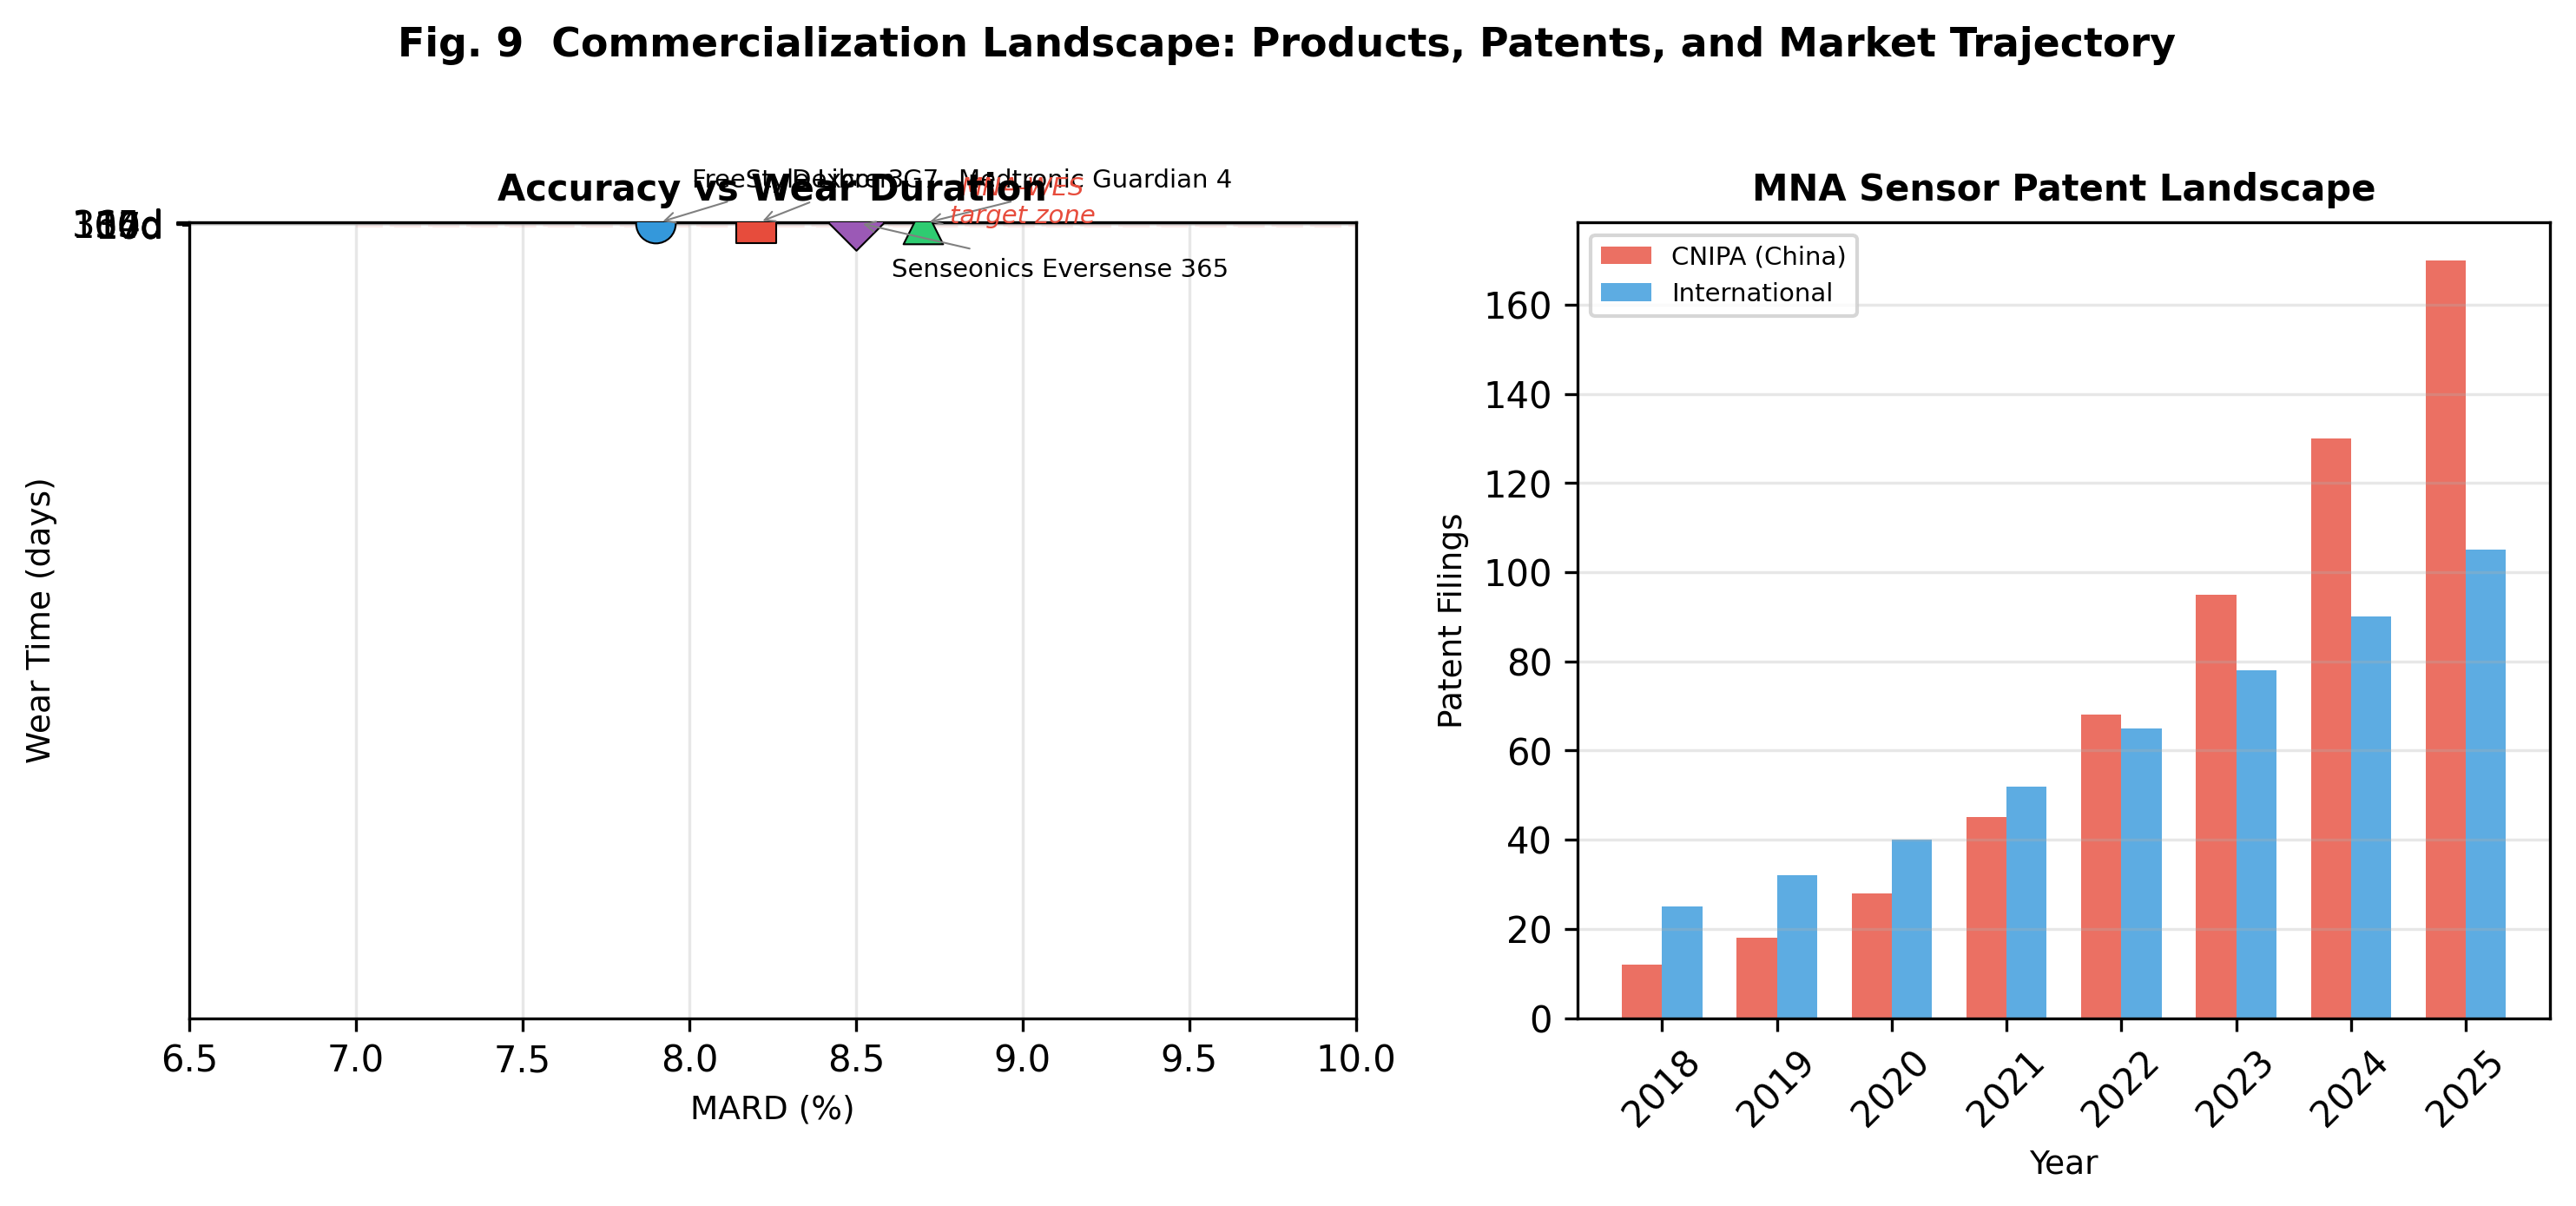
\includegraphics[width=\textwidth]{fig_09_commercial.png}
\caption{Commercialization landscape for MNA-based wearable electrochemical sensing. (Left) Accuracy (MARD) versus wear duration for commercial CGM products; the dashed red box indicates the MNA-WES target zone. (Right) MNA sensor patent filing trends (2018--2025) showing rapid growth in Chinese (CNIPA) filings.}
\label{fig:commercial}
\end{figure}

\subsection{Open Questions: 15 Unsolved Engineering Challenges}
\label{subsec:open_questions}

For researchers entering the field, Table~\ref{tab:open_questions} and Fig.~\ref{fig:open_questions} provide a prioritized list of 15 unresolved engineering challenges, each rated by research priority and difficulty level. These questions define the current research frontier and represent opportunities for high-impact contributions:

\begin{figure}[htbp]
\centering
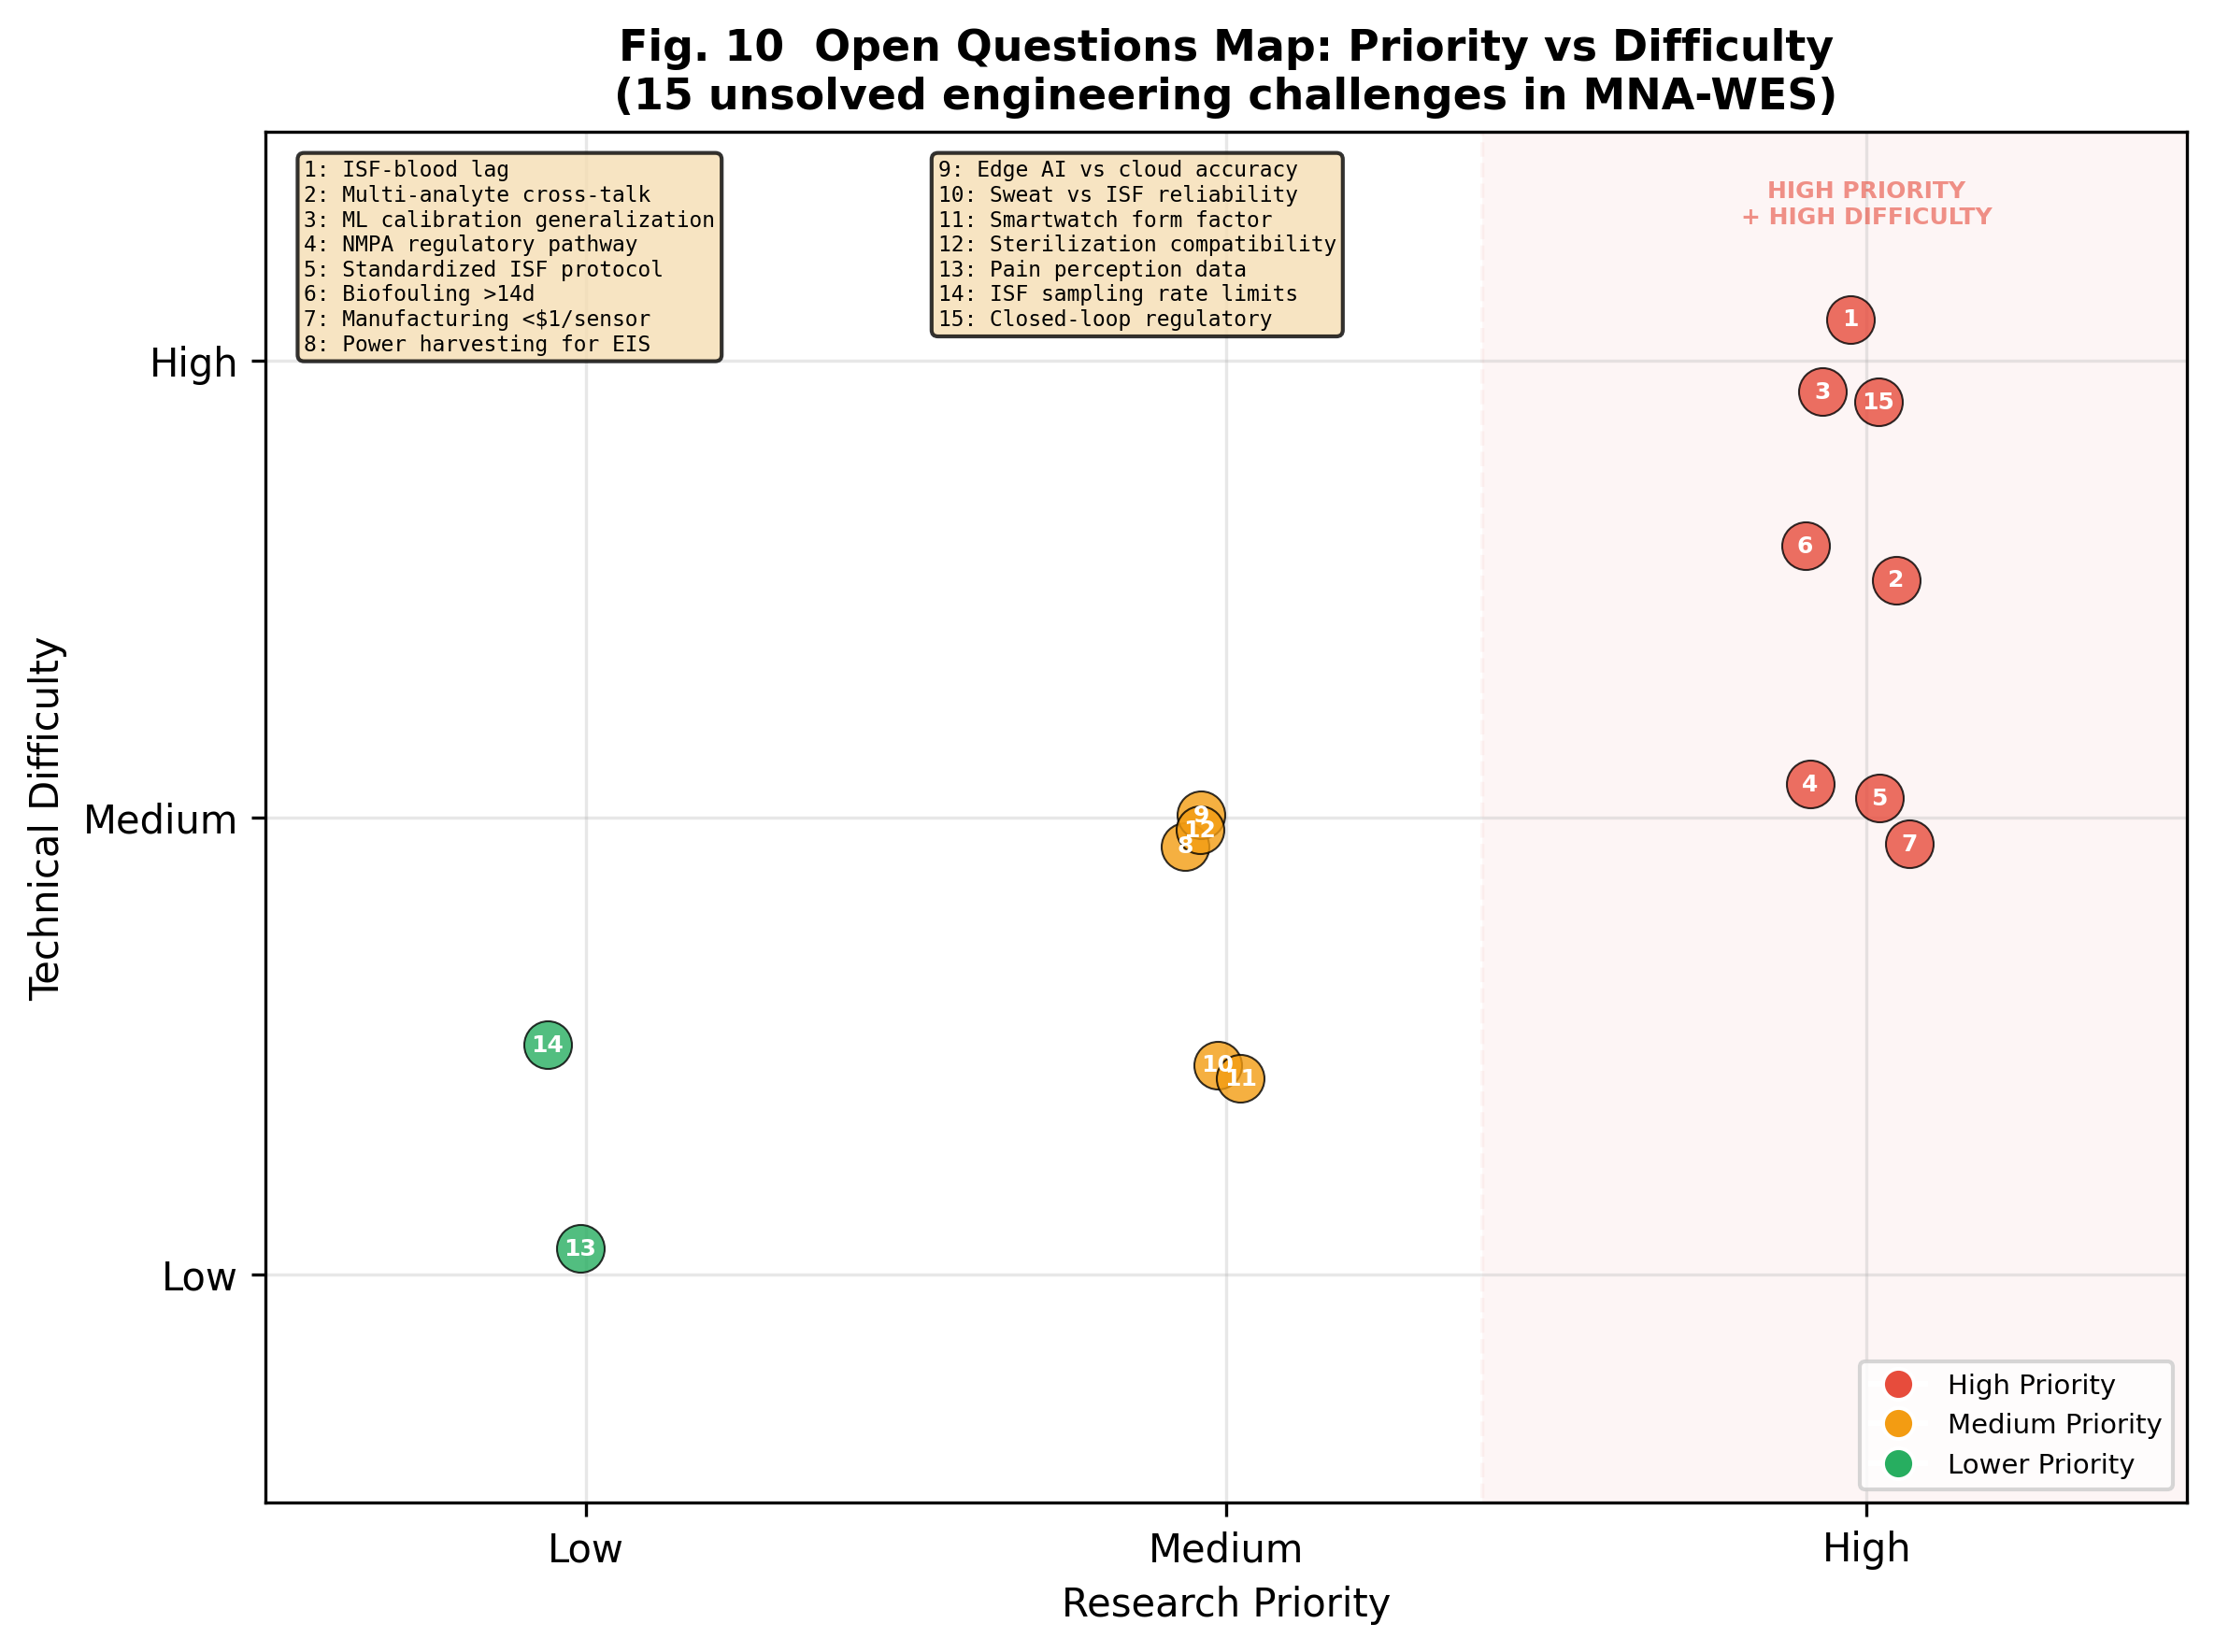
\includegraphics[width=0.8\textwidth]{fig_10_open_questions.png}
\caption{Open questions map: 15 unsolved engineering challenges in MNA-based wearable electrochemical sensing, plotted by research priority versus technical difficulty. Numbers correspond to Table~\ref{tab:open_questions}. The upper-right quadrant (high priority, high difficulty) represents the most impactful research opportunities.}
\label{fig:open_questions}
\end{figure}

\textit{High priority, high difficulty:}
(1) ISF-blood glucose lag: exact magnitude under exercise, fasting, and postprandial conditions remains disputed (5--20~min range); (2) Multi-analyte cross-talk minimization in dense multiplexed arrays; (3) Personalized ML calibration generalizable across diverse patient populations; (4) NMPA regulatory pathway for microneedle CGM in China.

\textit{High priority, medium difficulty:}
(5) Standardized ISF extraction protocol for reproducible cross-laboratory comparison; (6) Long-term biofouling mitigation beyond 14-day wear; (7) Manufacturing cost reduction to $<$\$1/sensor for consumer health market.

\textit{Medium priority, medium difficulty:}
(8) Power harvesting sufficient for continuous EIS measurement; (9) Edge AI inference accuracy vs.\ cloud-based processing; (10) Sweat vs.\ ISF: which biofluid is more reliable for continuous monitoring? (11) Integration with smartwatch/fitness tracker form factor; (12) Sterilization methods compatible with enzyme-functionalized needles.

\textit{Lower priority:}
(13) Microneedle pain perception: quantitative psychophysical data across skin types; (14) ISF sampling rate physiological limits; (15) Closed-loop therapy regulatory pathway for autonomous dosing decisions.


%%
%% SECTION 8: CONCLUSION
%%
\section{Conclusion}
\label{sec:conclusion}

This review has adopted a measurement instrument chain framework to systematically analyze MNA-based wearable electrochemical sensing as a complete engineering system — from microneedle material design through electrochemical transduction and signal chain integration to embedded intelligence and clinical translation — covering 200 papers from 2000 to 2026. Three conclusions are warranted:

First, the full-chain integration of MNA fabrication, electrochemical transduction, FPCB circuit design, and embedded intelligence has been demonstrated at the prototype level by multiple groups, with clinical validation in human subjects for glucose and lactate. The 14-day MARD of 10.2\% \cite{Yang2023CGM14day} and the 21-patient ISF lactate study \cite{Djassemi2026ACSsens} represent the current clinical state-of-the-art, establishing MNA-WES as a credible competitor to commercial CGM for the first time.

Second, multi-analyte multiplexed MNA systems with in-sensor computing — exemplified by the 9-analyte self-calibrating array \cite{Li2025Innovation} and the in-sensor metabolic assessment platform \cite{Fan2026EdgeAI} — define the next capability frontier. These systems move beyond single-biomarker monitoring toward holistic metabolic state assessment, with applications from personalized nutrition to real-time sepsis early warning.

Third, the translation gap from laboratory demonstration to cleared clinical device remains substantial. Biofouling-induced long-term stability, ISF-blood lag compensation, regulatory pathway navigation, and manufacturing cost reduction are the four rate-limiting challenges. Addressing these challenges will require interdisciplinary collaboration across electrochemistry, flexible electronics, embedded AI, clinical validation, and regulatory science — the exact combination this full-chain review framework is designed to foster.

%%
%% NEW TABLES ADDED IN v4.2.0 UPGRADE
%%

\begin{table}[htbp]
\centering
\small
\caption{MNA design decision guide: recommended material $\times$ geometry $\times$ fabrication method for common application scenarios. These guidelines are derived from the quantitative performance data in \S\ref{sec:fabrication}--\ref{sec:sensing} and serve as starting points for experimental design.}
\label{tab:design_guide}
\begin{tabular}{p{3.5cm}p{3cm}p{3cm}p{3cm}}
\toprule
\textbf{Application Scenario} & \textbf{Material} & \textbf{Geometry} & \textbf{Fabrication} \\
\midrule
Short-term single-analyte ($<$24~h) & SU-8 or PDMS & Solid, surface electrode & Micromolding \\
Long-term continuous ($>$7~d) & Stainless steel / Ti & Hollow, PEDOT matrix & Laser-cut + electrodeposition \\
Multi-analyte multiplexed & Si (DRIE) & Solid, zone-defined & Photolithography \\
Rapid prototyping & Photopolymer resin & Hollow, any geometry & DLP/SLA 3D printing \\
Dissolvable / drug dual & PVA / sugar & Coated solid & Cast molding \\
\bottomrule
\end{tabular}
\end{table}

\begin{table}[htbp]
\centering
\small
\caption{Quantitative comparison of electrochemical sensing modalities for MNA-based wearable systems. Performance ranges represent the span of values reported across the corpus of this review. Power figures assume single-channel operation with commercial or custom AFE.}
\label{tab:modality_comparison}
\begin{tabular}{p{2.2cm}cccccc}
\toprule
\textbf{Modality} & \textbf{Typical Analyte} & \textbf{LOD} & \textbf{Sensitivity} & \textbf{Response} & \textbf{Stability} & \textbf{Power} \\
\midrule
Amperometry & Glucose, lactate & 0.1--5~$\mu$M & 10--200~$\mu$A~mM$^{-1}$~cm$^{-2}$ & $<$30~s & 7--14~d & $\sim$1~mW \\
DPV / SWV & Uric acid, drugs & 0.01--1~$\mu$M & --- & $<$60~s & --- & $\sim$5~mW \\
EIS & Cortisol, proteins & 0.01--1~ng~mL$^{-1}$ & --- & 5--30~min & --- & $\sim$0.5~mW \\
Potentiometry (ISE) & Na$^+$, K$^+$, pH & --- & 55--62~mV~dec$^{-1}$ & $<$10~s & $>$30~d & $\sim$0.1~mW \\
FSCV & Dopamine & 1--10~nM & --- & $<$1~s & --- & $\sim$10~mW \\
\bottomrule
\end{tabular}
\end{table}

\begin{table}[htbp]
\centering
\small
\caption{Commercial CGM product comparison. MARD values from published clinical studies; wear durations from manufacturer specifications. These products represent the current clinical gold standard against which MNA-WES prototypes are benchmarked.}
\label{tab:commercial}
\begin{tabular}{lcccc}
\toprule
\textbf{Product} & \textbf{MARD (\%)} & \textbf{Wear Time} & \textbf{Sensor Type} & \textbf{Regulatory} \\
\midrule
Dexcom G7 & 8.2 & 10~d & Enzyme electrode & FDA 510(k) \\
FreeStyle Libre 3 & 7.9 & 14~d & Enzyme electrode & FDA 510(k) + CE \\
Medtronic Guardian 4 & 8.7 & 7~d & Enzyme electrode & FDA 510(k) \\
Senseonics Eversense 365 & 8.5 & 365~d & Fluorescence & FDA PMA \\
\bottomrule
\end{tabular}
\end{table}

\begin{table}[htbp]
\centering
\small
\caption{Fifteen open engineering challenges in MNA-based wearable electrochemical sensing, prioritized by research importance and difficulty. These questions define the current research frontier and represent high-impact contribution opportunities for newcomers to the field.}
\label{tab:open_questions}
\begin{tabular}{clll}
\toprule
\textbf{\#} & \textbf{Challenge} & \textbf{Priority} & \textbf{Difficulty} \\
\midrule
1 & ISF-blood glucose lag under varying conditions & High & Clinical validation \\
2 & Multi-analyte cross-talk minimization & High & Sensor design \\
3 & Personalized ML calibration generalizability & High & Data science \\
4 & NMPA regulatory pathway for MN CGM in China & High & Regulatory \\
5 & Standardized ISF extraction protocol & High & Methodology \\
6 & Biofouling mitigation beyond 14-day wear & High & Materials \\
7 & Manufacturing cost $<$\$1/sensor & High & Manufacturing \\
8 & Power harvesting for continuous EIS & Medium & Circuit design \\
9 & Edge AI vs.\ cloud accuracy trade-off & Medium & Embedded systems \\
10 & Sweat vs.\ ISF reliability comparison & Medium & Physiology \\
11 & Smartwatch form factor integration & Medium & Industrial design \\
12 & Sterilization of enzyme-functionalized needles & Medium & Manufacturing \\
13 & Pain perception across skin types & Low & Clinical \\
14 & ISF sampling rate physiological limits & Low & Physiology \\
15 & Closed-loop therapy regulatory pathway & High & Regulatory \\
\bottomrule
\end{tabular}
\end{table}


%%
%% CREDIT AUTHORSHIP
%%
\section*{CRediT authorship contribution statement}
\textbf{Yuanjie Zhang}: Conceptualization, Methodology, Writing -- Original Draft (all sections), Visualization, Formal analysis.
\textbf{Kan Wang}: Conceptualization, Supervision, Funding acquisition, Writing -- Review \& Editing, Project administration.

%%
%% DECLARATIONS
%%
\section*{Declaration of competing interests}
The authors declare that they have no known competing financial interests or personal relationships that could have appeared to influence the work reported in this paper.

\section*{Data availability}
No new data were generated or analyzed during the preparation of this review article.

\section*{Acknowledgments}
This work was supported by the National Natural Science Foundation of China (Grant No. [XXXXXXXX]) and the Shanghai Jiao Tong University Research Fund (Grant No. [XXXXXXXX]). The authors thank members of the Wang Lab at the School of Automation and Sensing Science and Engineering, SJTU, for valuable discussions.

%%
%% BIBLIOGRAPHY
%%
\clearpage
\bibliographystyle{elsarticle-num}
\bibliography{references}

%%
%% FIGURES — place after bibliography per B&B requirements
%%
\begin{figure}[h]
\centering
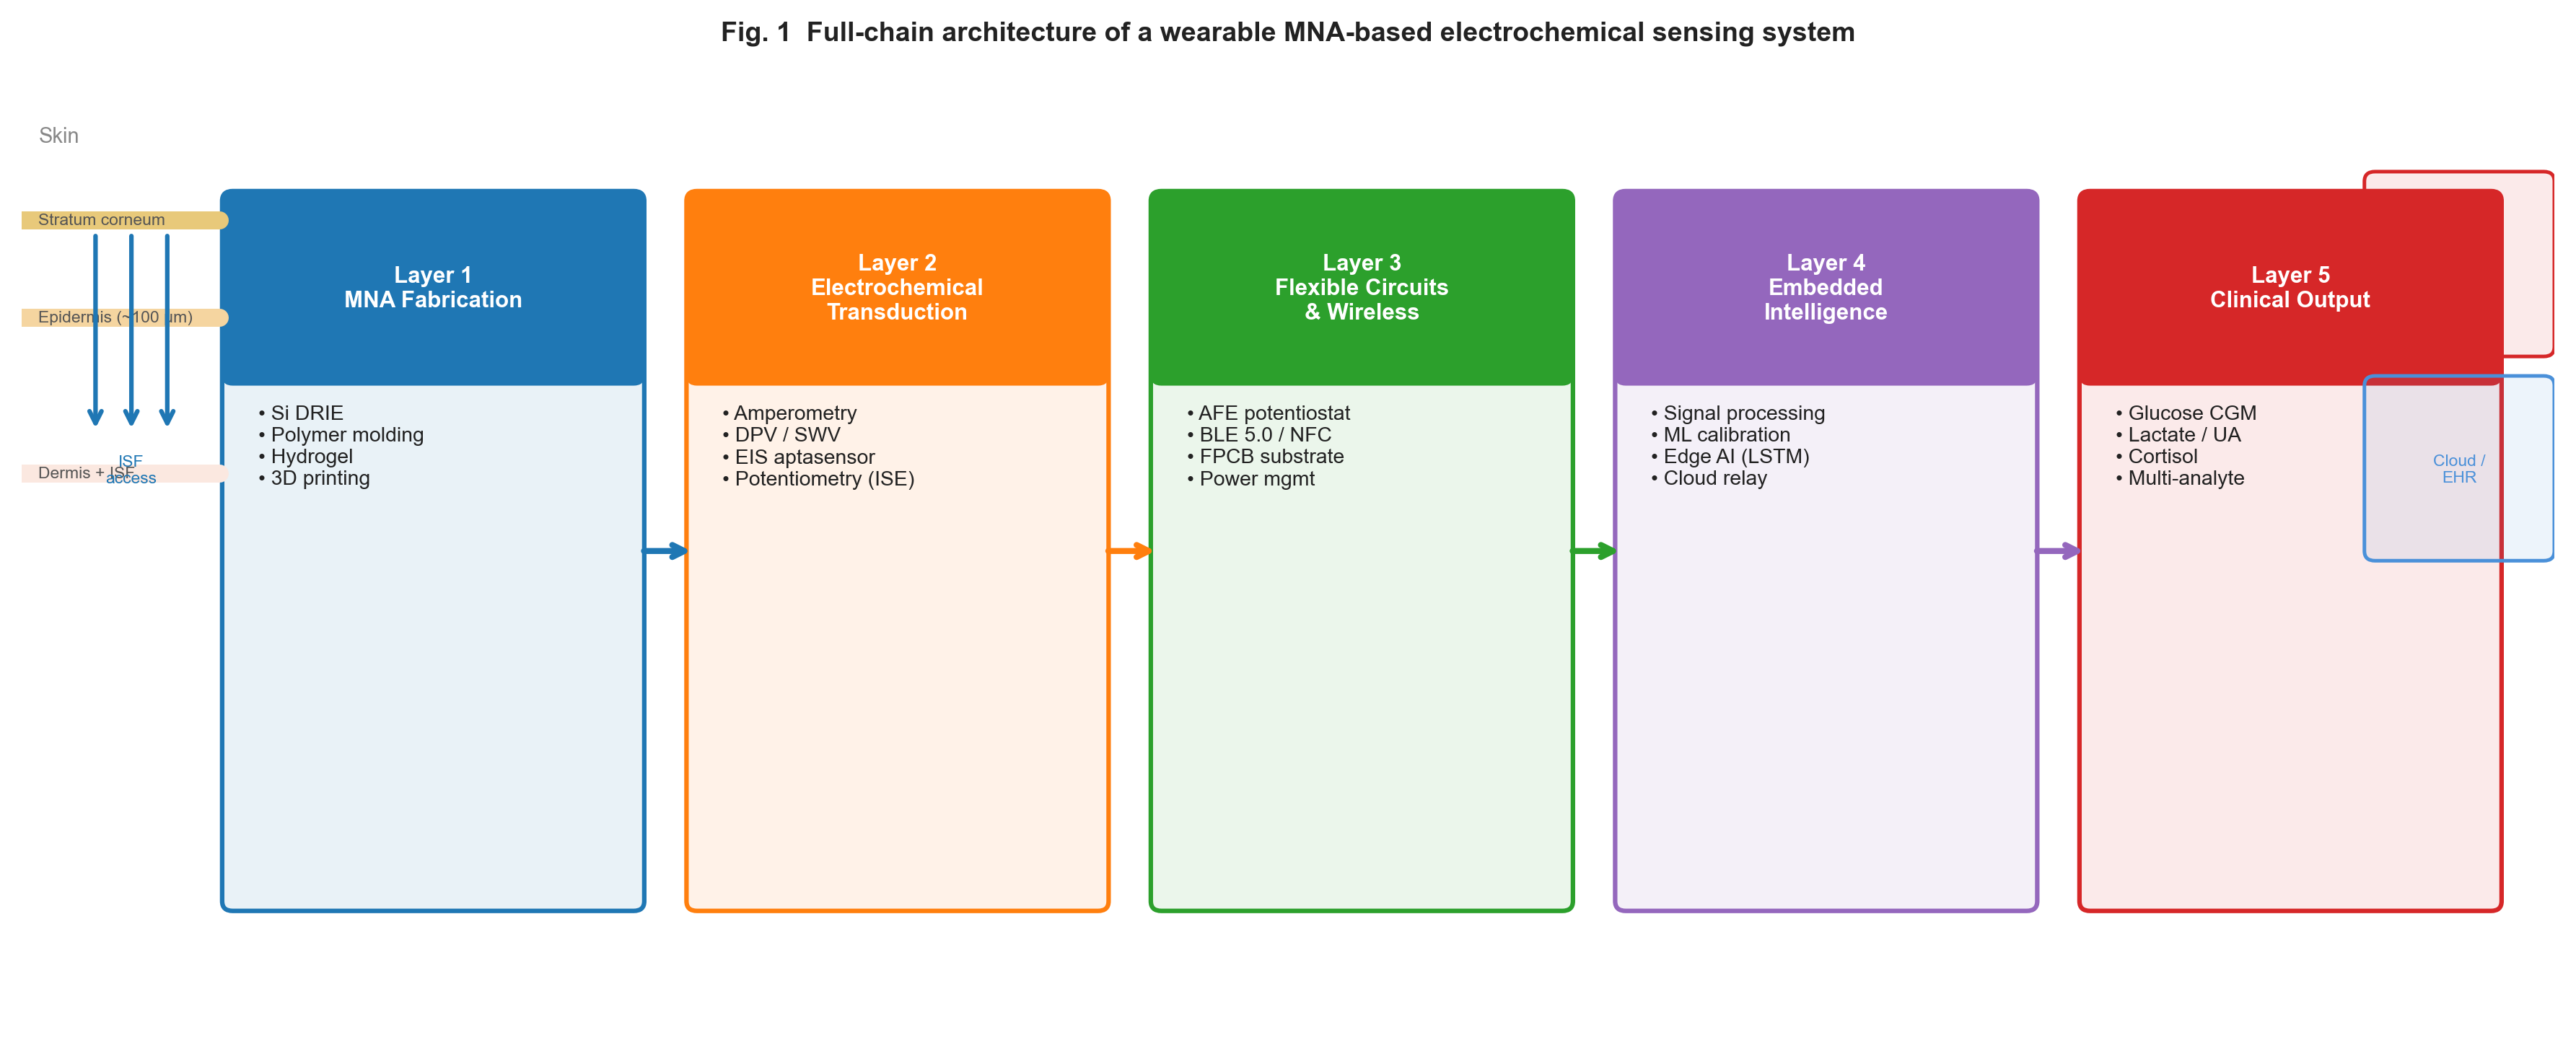
\includegraphics[width=\textwidth]{fig_01_system_chain.png}
\caption{Full-chain architecture of a wearable microneedle array-based electrochemical sensing system. The five engineering layers — (1) MNA fabrication, (2) electrochemical transduction, (3) signal conditioning and wireless transmission, (4) embedded intelligent processing, and (5) clinical output — are reviewed systematically in Sections~2--6, respectively.}
\label{fig:system_chain}
\end{figure}

\begin{figure}[h]
\centering
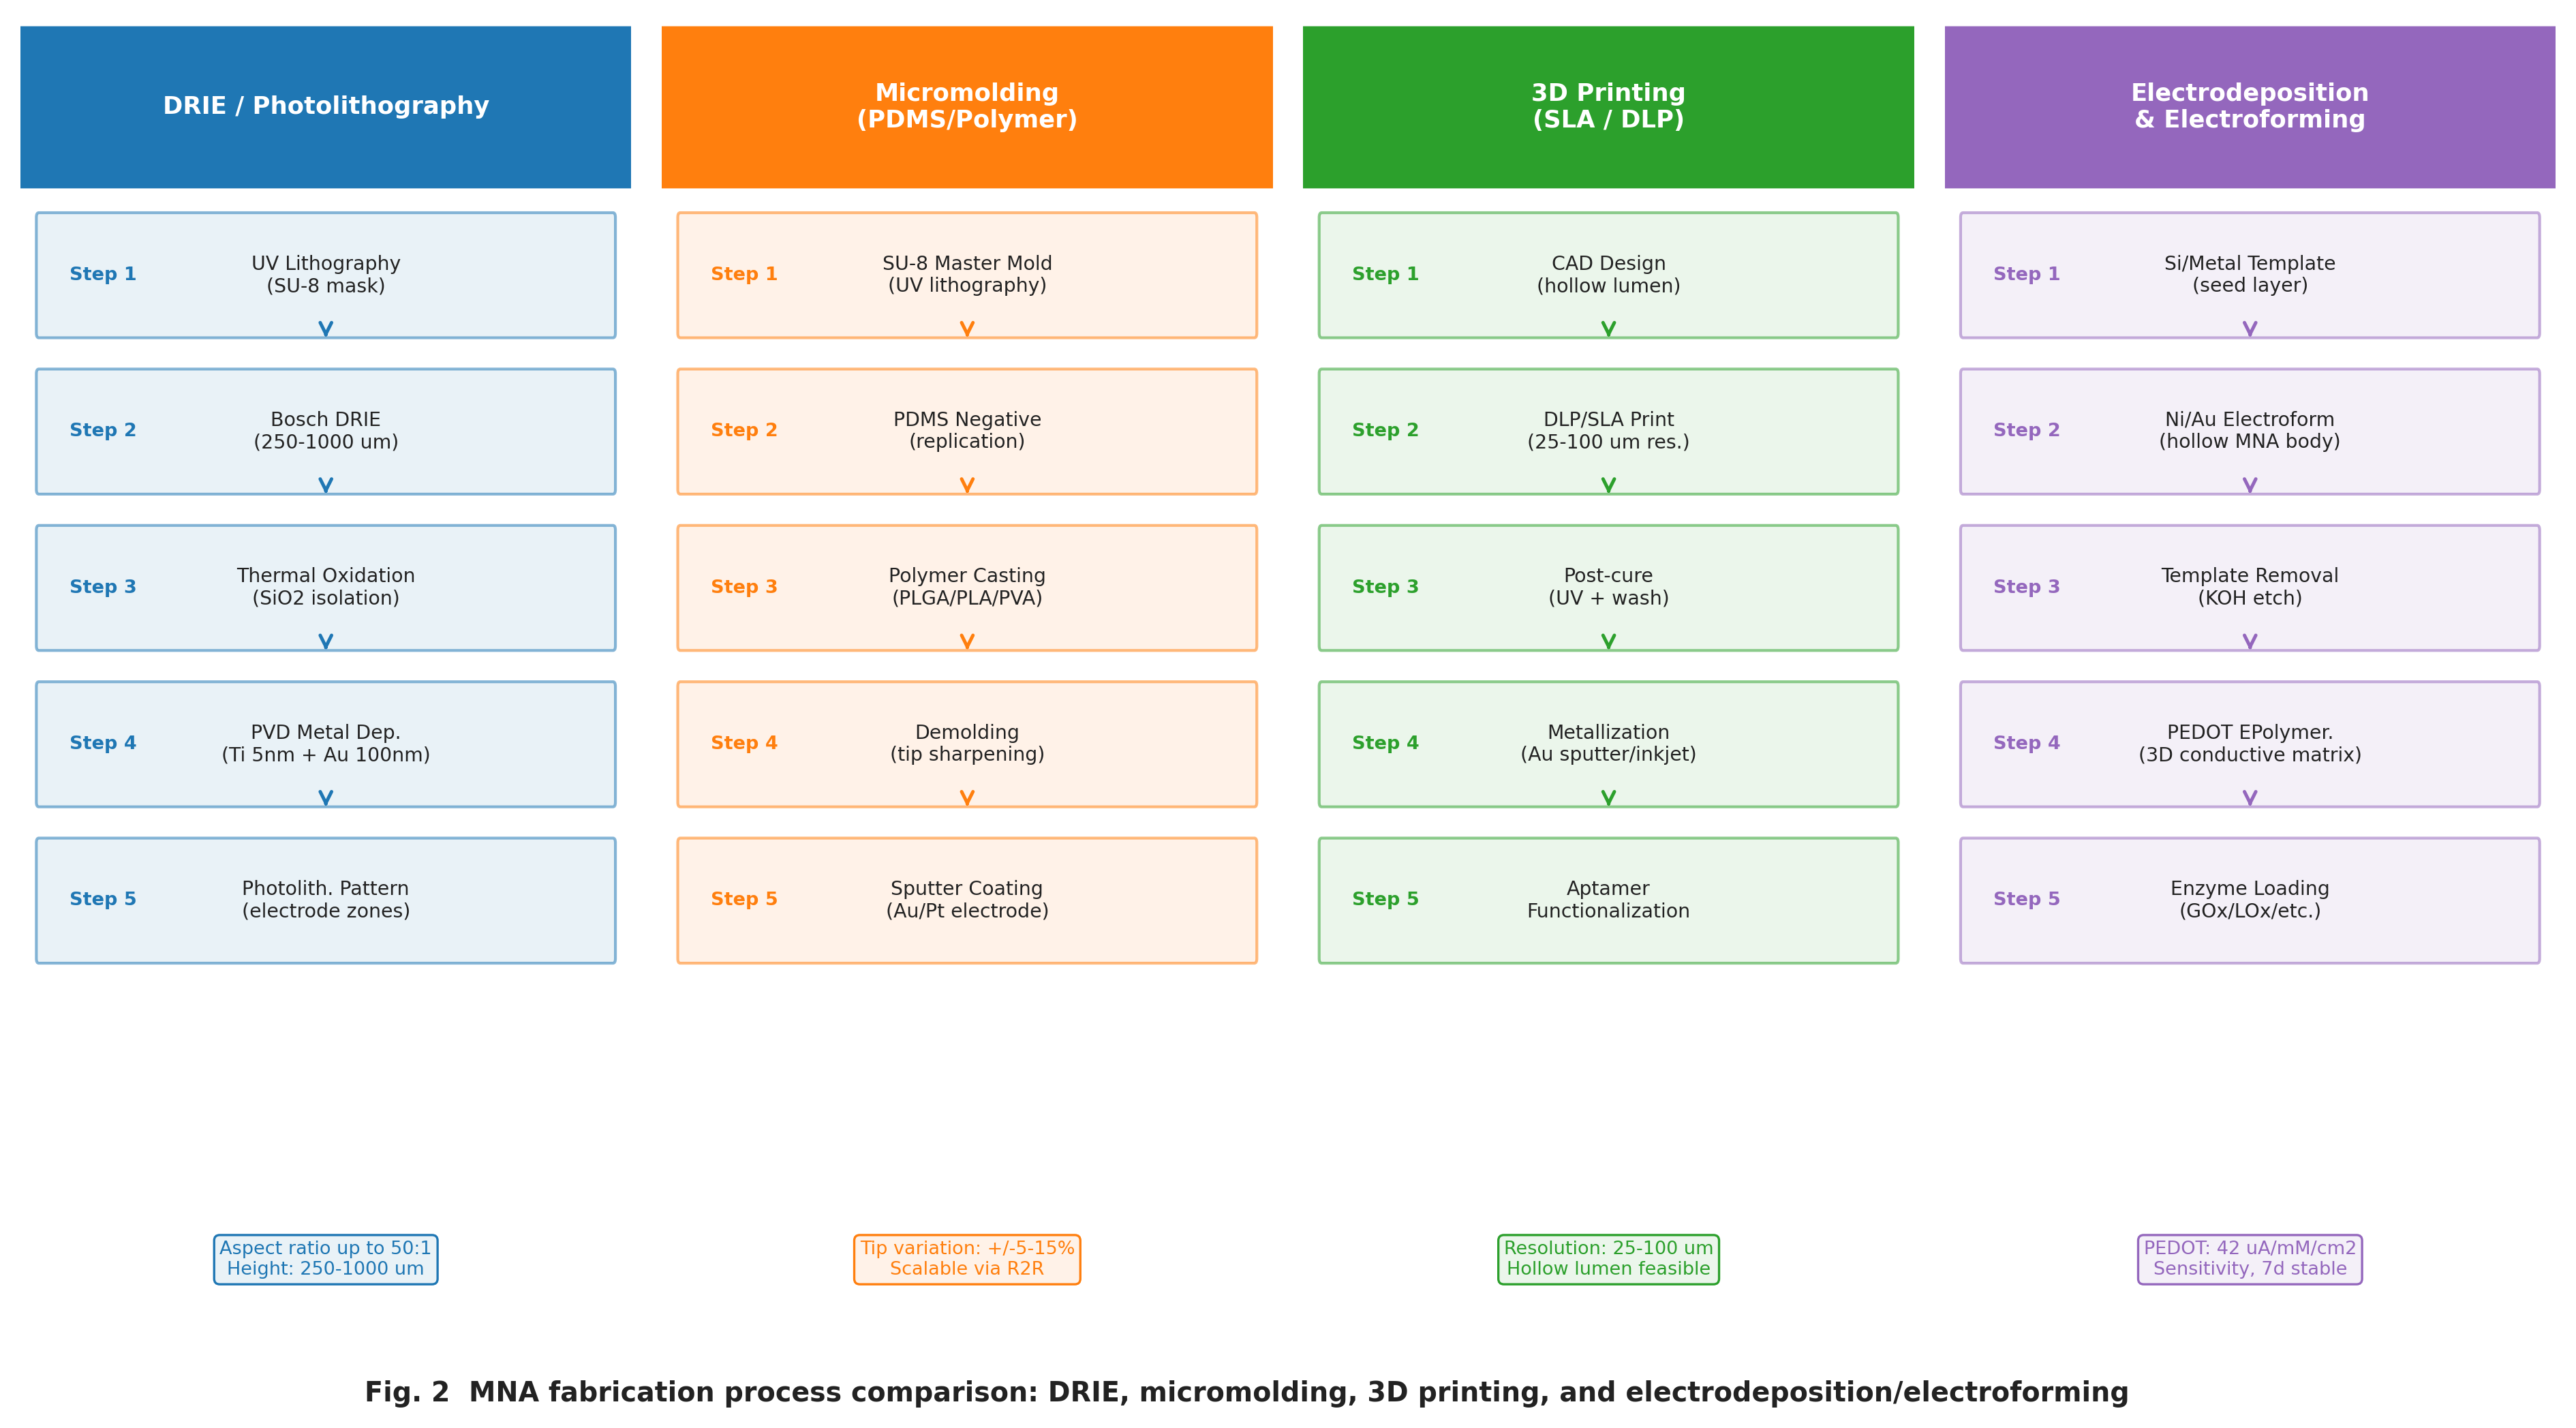
\includegraphics[width=\textwidth]{fig_02_fabrication.png}
\caption{Microneedle array fabrication process comparison. Four principal routes: (a)~silicon DRIE/photolithography, (b)~polymer micromolding (PDMS/SU-8), (c)~3D printing (SLA/DLP), and (d)~electrodeposition and electroforming. Representative process steps, dimensional specifications, and key performance metrics are shown for each route.}
\label{fig:fabrication}
\end{figure}

\begin{figure}[h]
\centering
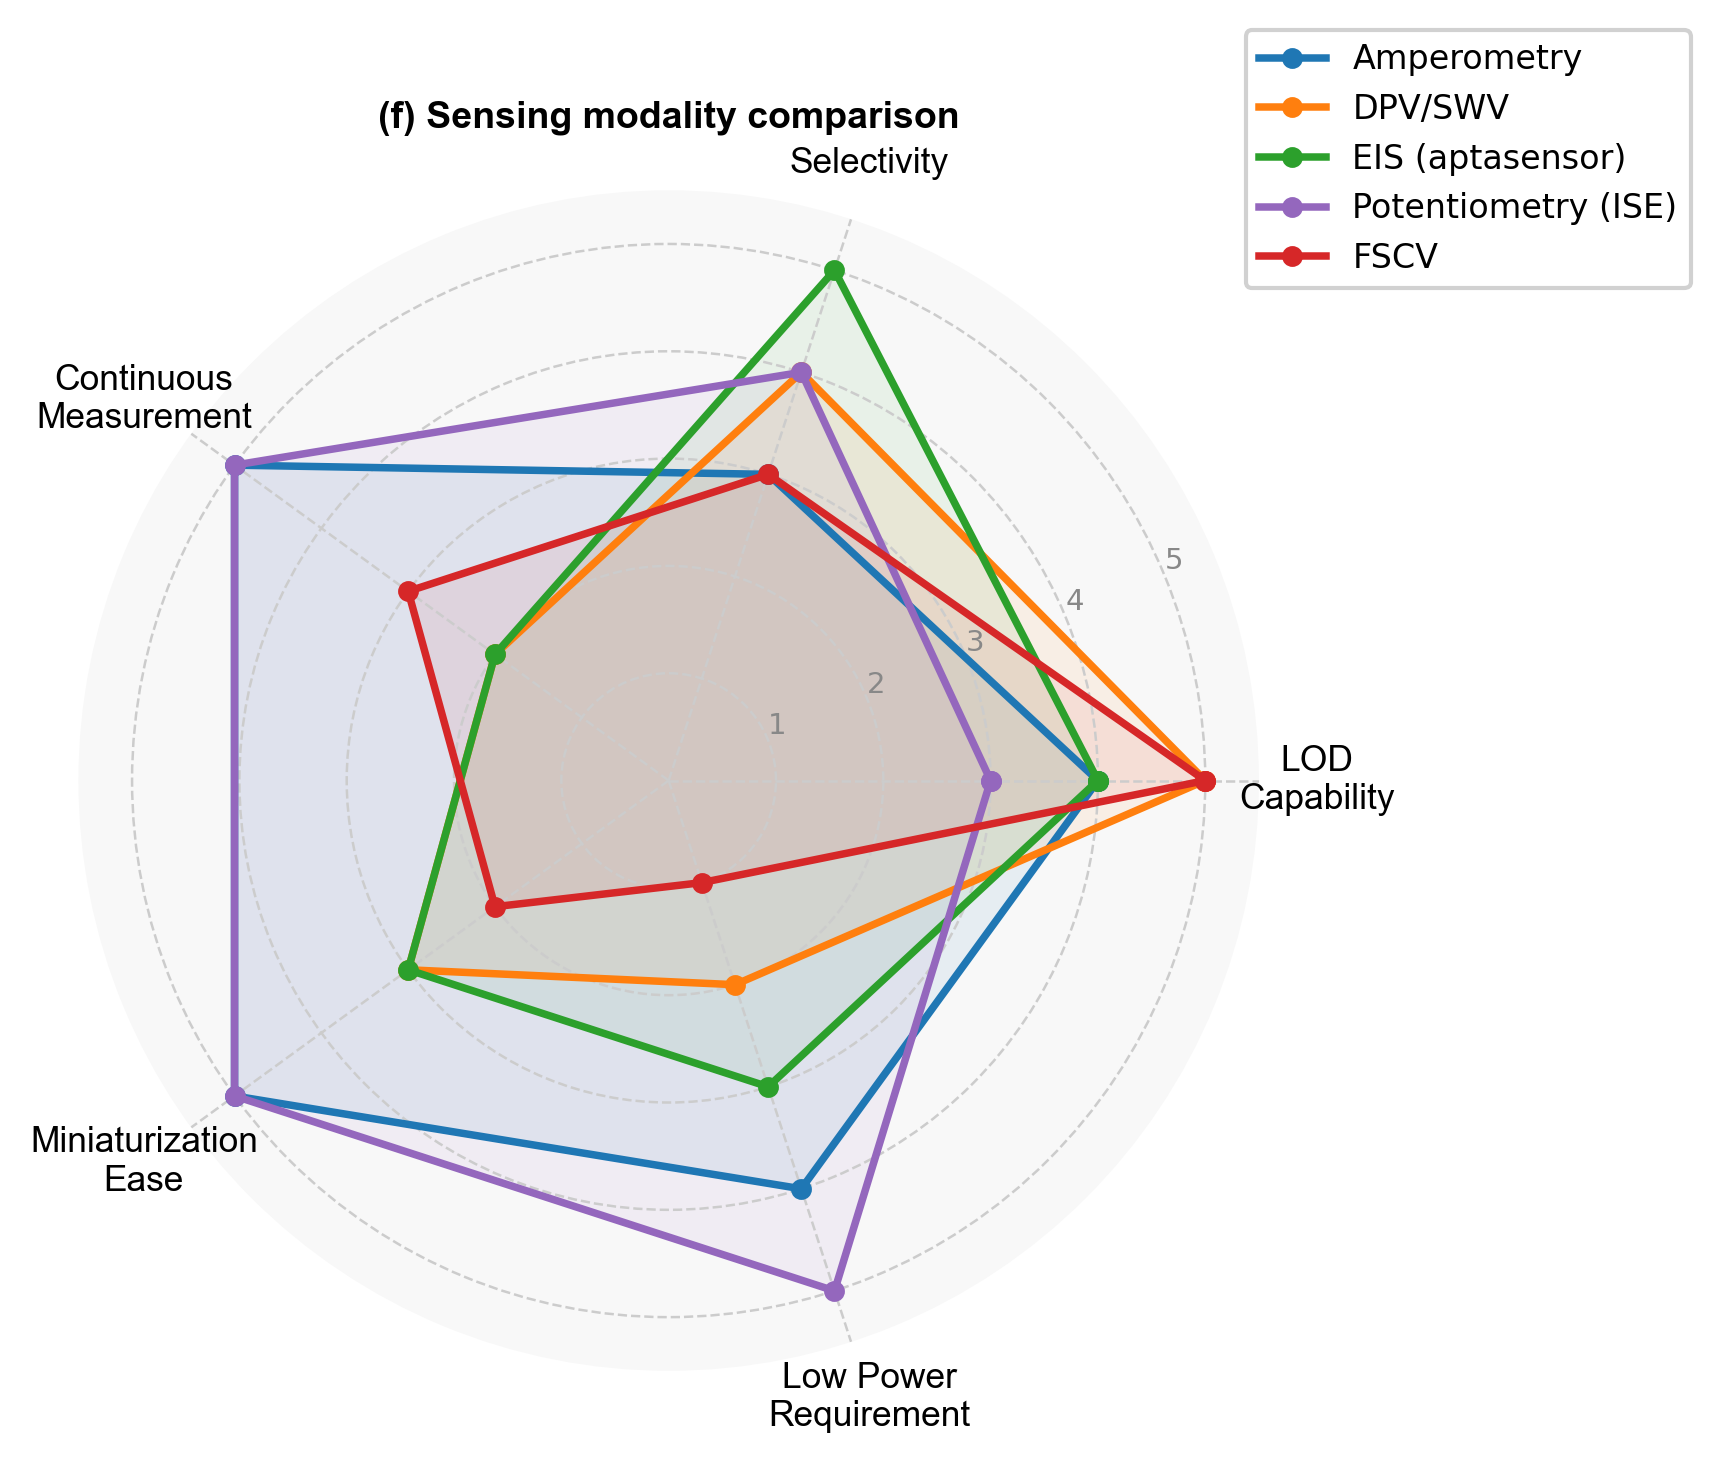
\includegraphics[width=0.5\textwidth]{fig_03_modality_radar.png}
\caption{Electrochemical sensing modalities for MNA-based wearable sensors. (a) Amperometric i--t response. (b) Differential pulse voltammogram. (c) EIS Nyquist plot pre- and post-target binding. (d) Nernstian potentiometric response for K\textsuperscript{+}. (e) FSCV color plot for dopamine detection. (f) Multi-axis modality comparison.}
\label{fig:sensing}
\end{figure}

\begin{figure}[h]
\centering
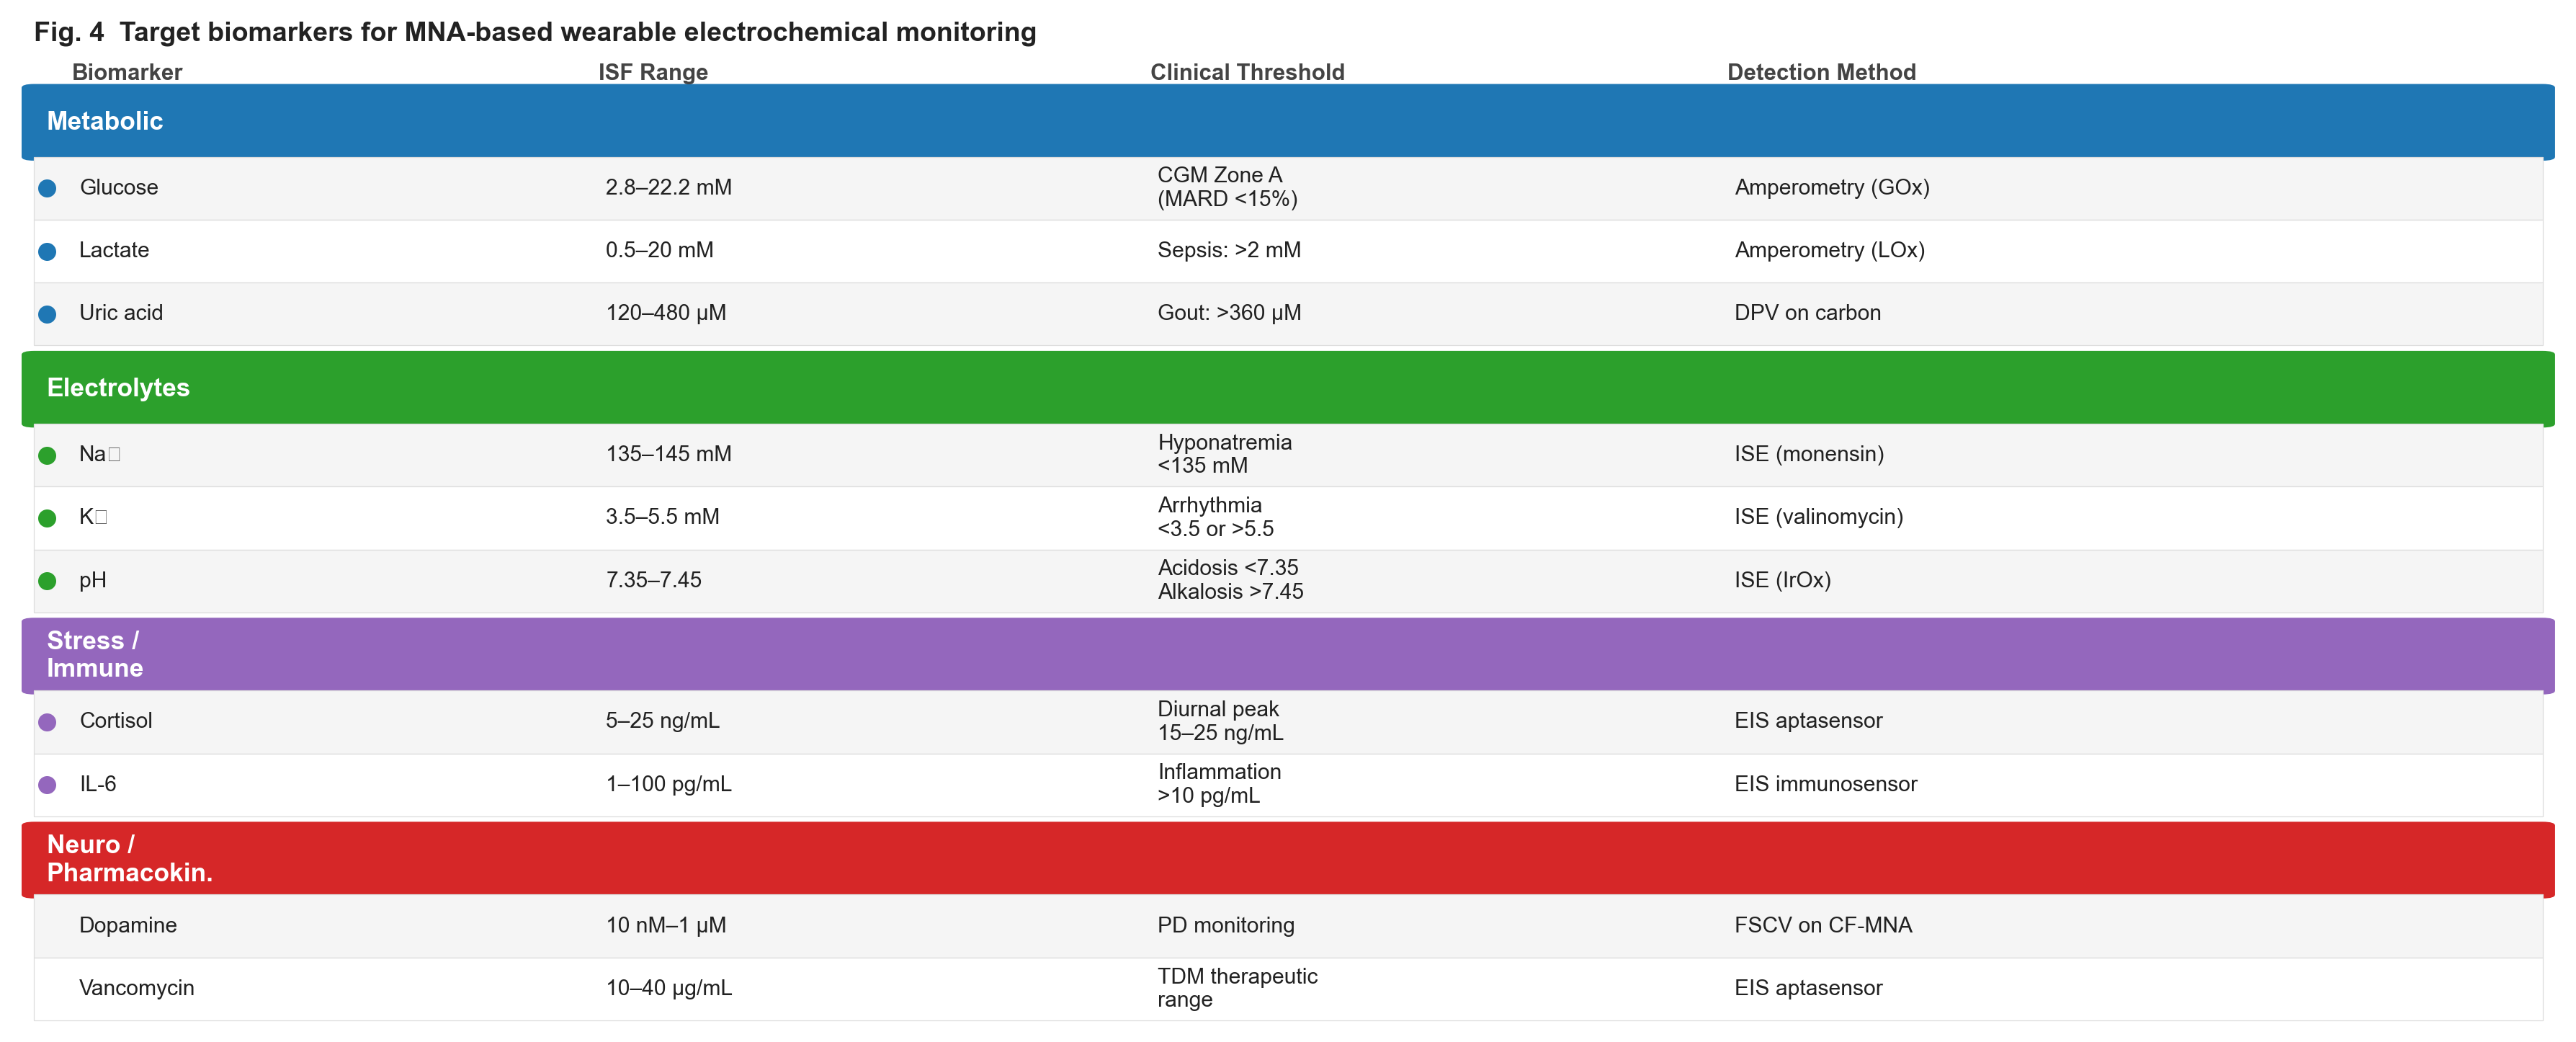
\includegraphics[width=\textwidth]{fig_04_biomarkers.png}
\caption{Target biomarkers for MNA-based wearable electrochemical monitoring. Clinical ISF concentration ranges, alarm thresholds, and applicable detection modalities are indicated for each analyte category.}
\label{fig:biomarkers}
\end{figure}

\begin{figure}[h]
\centering
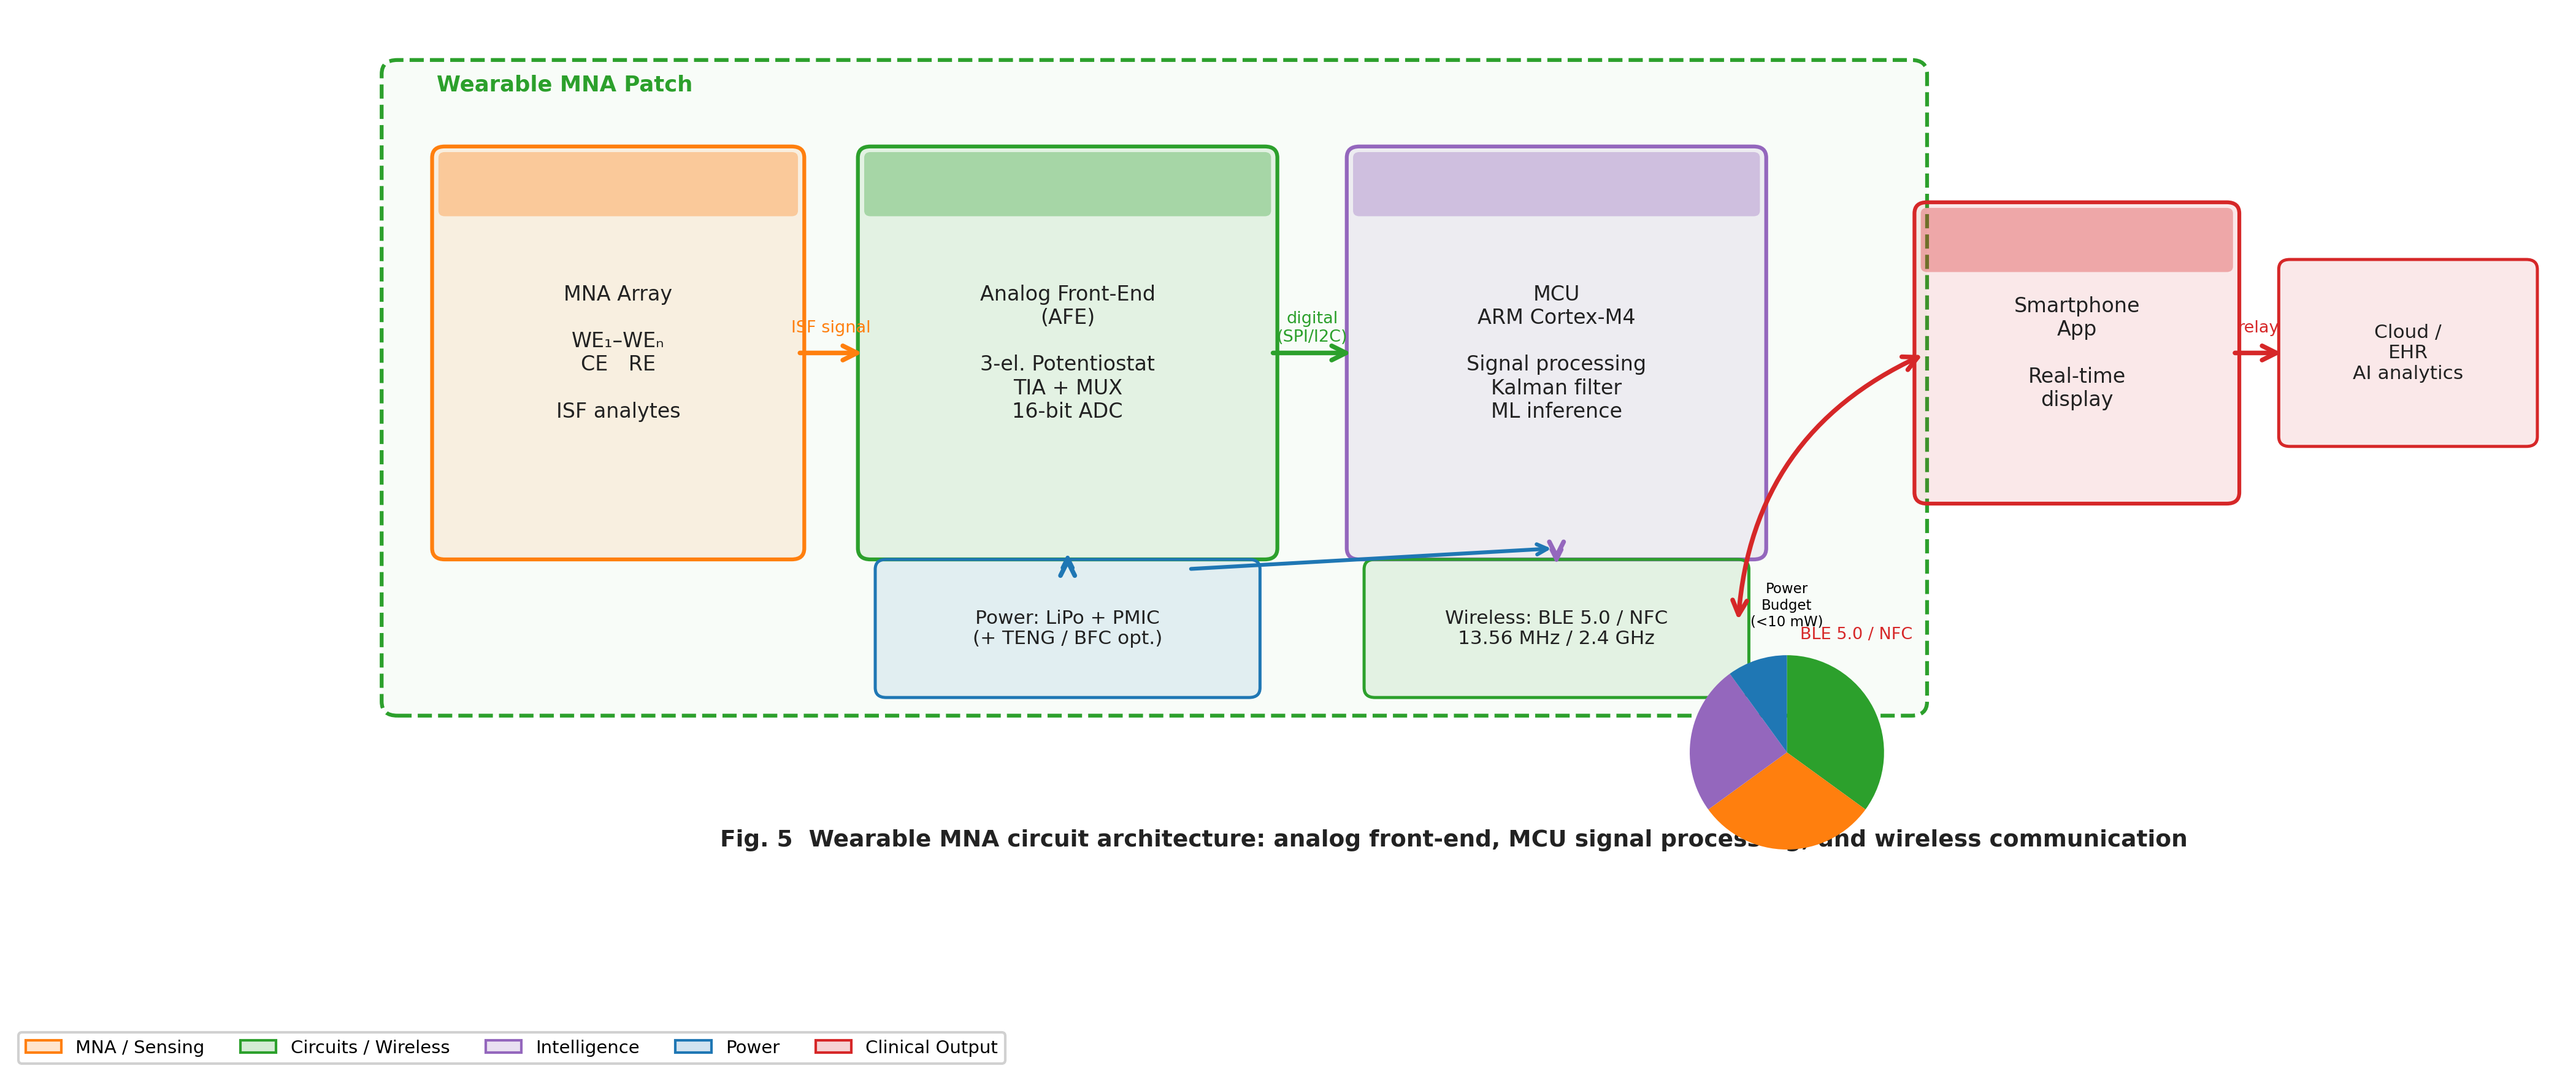
\includegraphics[width=\textwidth]{fig_05_circuits.png}
\caption{Wearable circuit architecture for MNA electrochemical sensing. Complete system block diagram from MNA transducer through analog front-end (AFE), MCU signal processing, wireless communication (BLE~5.0/NFC), to smartphone app and cloud/EHR relay. Inset: system power budget breakdown ($<$10~mW total target).}
\label{fig:circuits}
\end{figure}

\begin{figure}[h]
\centering
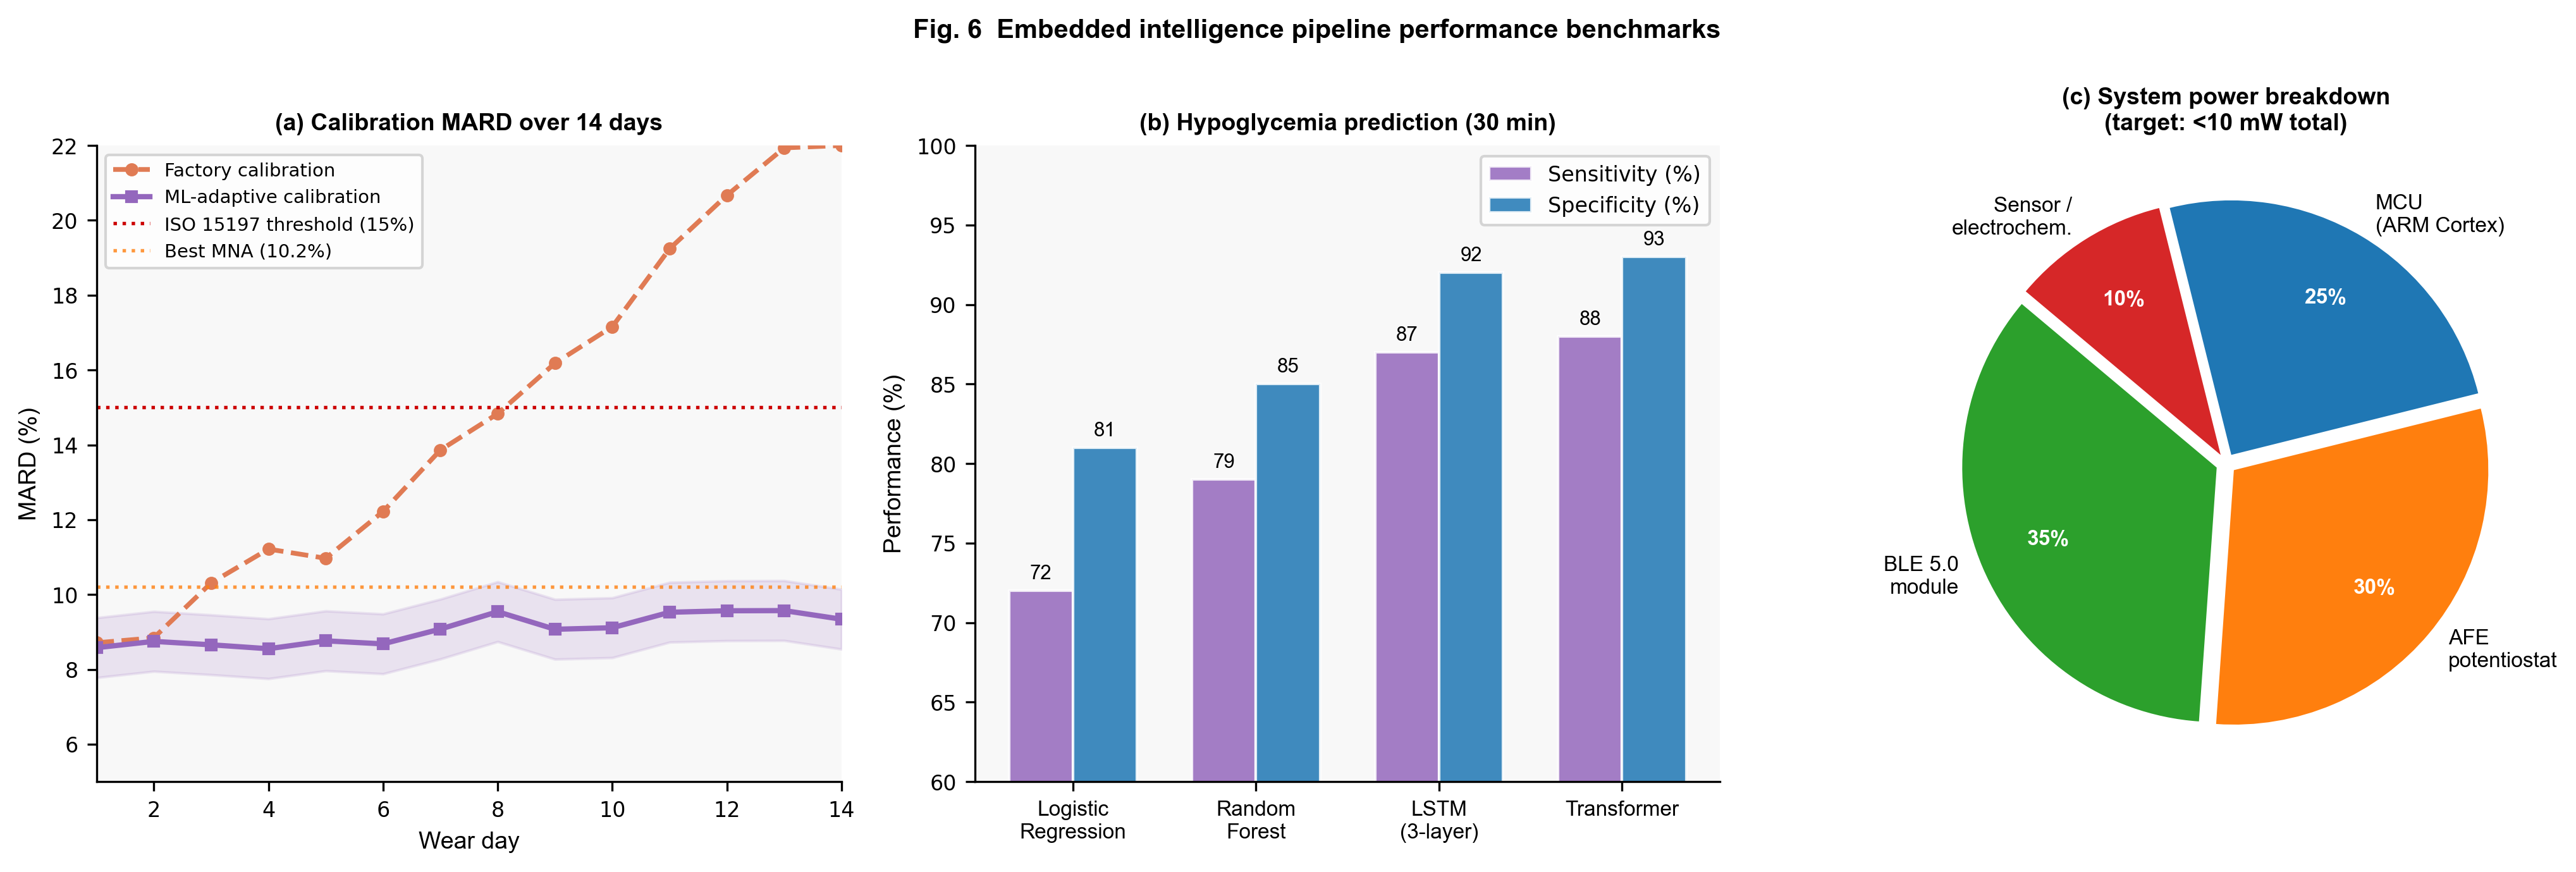
\includegraphics[width=\textwidth]{fig_06_intelligence.png}
\caption{Embedded intelligence pipeline for wearable MNA sensing. (a) MARD comparison between factory and ML-adaptive calibration. (b) Hypoglycemia prediction accuracy. (c) System power breakdown.}
\label{fig:intelligence}
\end{figure}

\end{document}
